\documentclass[]{book}
\usepackage{lmodern}
\usepackage{amssymb,amsmath}
\usepackage{ifxetex,ifluatex}
\usepackage{fixltx2e} % provides \textsubscript
\ifnum 0\ifxetex 1\fi\ifluatex 1\fi=0 % if pdftex
  \usepackage[T1]{fontenc}
  \usepackage[utf8]{inputenc}
\else % if luatex or xelatex
  \ifxetex
    \usepackage{mathspec}
  \else
    \usepackage{fontspec}
  \fi
  \defaultfontfeatures{Ligatures=TeX,Scale=MatchLowercase}
\fi
% use upquote if available, for straight quotes in verbatim environments
\IfFileExists{upquote.sty}{\usepackage{upquote}}{}
% use microtype if available
\IfFileExists{microtype.sty}{%
\usepackage{microtype}
\UseMicrotypeSet[protrusion]{basicmath} % disable protrusion for tt fonts
}{}
\usepackage{hyperref}
\hypersetup{unicode=true,
            pdftitle={R, Rstudio, and ggplot2},
            pdfauthor={Sunbok Lee},
            pdfborder={0 0 0},
            breaklinks=true}
\urlstyle{same}  % don't use monospace font for urls
\usepackage{natbib}
\bibliographystyle{apalike}
\usepackage{color}
\usepackage{fancyvrb}
\newcommand{\VerbBar}{|}
\newcommand{\VERB}{\Verb[commandchars=\\\{\}]}
\DefineVerbatimEnvironment{Highlighting}{Verbatim}{commandchars=\\\{\}}
% Add ',fontsize=\small' for more characters per line
\usepackage{framed}
\definecolor{shadecolor}{RGB}{248,248,248}
\newenvironment{Shaded}{\begin{snugshade}}{\end{snugshade}}
\newcommand{\KeywordTok}[1]{\textcolor[rgb]{0.13,0.29,0.53}{\textbf{{#1}}}}
\newcommand{\DataTypeTok}[1]{\textcolor[rgb]{0.13,0.29,0.53}{{#1}}}
\newcommand{\DecValTok}[1]{\textcolor[rgb]{0.00,0.00,0.81}{{#1}}}
\newcommand{\BaseNTok}[1]{\textcolor[rgb]{0.00,0.00,0.81}{{#1}}}
\newcommand{\FloatTok}[1]{\textcolor[rgb]{0.00,0.00,0.81}{{#1}}}
\newcommand{\ConstantTok}[1]{\textcolor[rgb]{0.00,0.00,0.00}{{#1}}}
\newcommand{\CharTok}[1]{\textcolor[rgb]{0.31,0.60,0.02}{{#1}}}
\newcommand{\SpecialCharTok}[1]{\textcolor[rgb]{0.00,0.00,0.00}{{#1}}}
\newcommand{\StringTok}[1]{\textcolor[rgb]{0.31,0.60,0.02}{{#1}}}
\newcommand{\VerbatimStringTok}[1]{\textcolor[rgb]{0.31,0.60,0.02}{{#1}}}
\newcommand{\SpecialStringTok}[1]{\textcolor[rgb]{0.31,0.60,0.02}{{#1}}}
\newcommand{\ImportTok}[1]{{#1}}
\newcommand{\CommentTok}[1]{\textcolor[rgb]{0.56,0.35,0.01}{\textit{{#1}}}}
\newcommand{\DocumentationTok}[1]{\textcolor[rgb]{0.56,0.35,0.01}{\textbf{\textit{{#1}}}}}
\newcommand{\AnnotationTok}[1]{\textcolor[rgb]{0.56,0.35,0.01}{\textbf{\textit{{#1}}}}}
\newcommand{\CommentVarTok}[1]{\textcolor[rgb]{0.56,0.35,0.01}{\textbf{\textit{{#1}}}}}
\newcommand{\OtherTok}[1]{\textcolor[rgb]{0.56,0.35,0.01}{{#1}}}
\newcommand{\FunctionTok}[1]{\textcolor[rgb]{0.00,0.00,0.00}{{#1}}}
\newcommand{\VariableTok}[1]{\textcolor[rgb]{0.00,0.00,0.00}{{#1}}}
\newcommand{\ControlFlowTok}[1]{\textcolor[rgb]{0.13,0.29,0.53}{\textbf{{#1}}}}
\newcommand{\OperatorTok}[1]{\textcolor[rgb]{0.81,0.36,0.00}{\textbf{{#1}}}}
\newcommand{\BuiltInTok}[1]{{#1}}
\newcommand{\ExtensionTok}[1]{{#1}}
\newcommand{\PreprocessorTok}[1]{\textcolor[rgb]{0.56,0.35,0.01}{\textit{{#1}}}}
\newcommand{\AttributeTok}[1]{\textcolor[rgb]{0.77,0.63,0.00}{{#1}}}
\newcommand{\RegionMarkerTok}[1]{{#1}}
\newcommand{\InformationTok}[1]{\textcolor[rgb]{0.56,0.35,0.01}{\textbf{\textit{{#1}}}}}
\newcommand{\WarningTok}[1]{\textcolor[rgb]{0.56,0.35,0.01}{\textbf{\textit{{#1}}}}}
\newcommand{\AlertTok}[1]{\textcolor[rgb]{0.94,0.16,0.16}{{#1}}}
\newcommand{\ErrorTok}[1]{\textcolor[rgb]{0.64,0.00,0.00}{\textbf{{#1}}}}
\newcommand{\NormalTok}[1]{{#1}}
\usepackage{longtable,booktabs}
\usepackage{graphicx,grffile}
\makeatletter
\def\maxwidth{\ifdim\Gin@nat@width>\linewidth\linewidth\else\Gin@nat@width\fi}
\def\maxheight{\ifdim\Gin@nat@height>\textheight\textheight\else\Gin@nat@height\fi}
\makeatother
% Scale images if necessary, so that they will not overflow the page
% margins by default, and it is still possible to overwrite the defaults
% using explicit options in \includegraphics[width, height, ...]{}
\setkeys{Gin}{width=\maxwidth,height=\maxheight,keepaspectratio}
\IfFileExists{parskip.sty}{%
\usepackage{parskip}
}{% else
\setlength{\parindent}{0pt}
\setlength{\parskip}{6pt plus 2pt minus 1pt}
}
\setlength{\emergencystretch}{3em}  % prevent overfull lines
\providecommand{\tightlist}{%
  \setlength{\itemsep}{0pt}\setlength{\parskip}{0pt}}
\setcounter{secnumdepth}{5}
% Redefines (sub)paragraphs to behave more like sections
\ifx\paragraph\undefined\else
\let\oldparagraph\paragraph
\renewcommand{\paragraph}[1]{\oldparagraph{#1}\mbox{}}
\fi
\ifx\subparagraph\undefined\else
\let\oldsubparagraph\subparagraph
\renewcommand{\subparagraph}[1]{\oldsubparagraph{#1}\mbox{}}
\fi

%%% Use protect on footnotes to avoid problems with footnotes in titles
\let\rmarkdownfootnote\footnote%
\def\footnote{\protect\rmarkdownfootnote}

%%% Change title format to be more compact
\usepackage{titling}

% Create subtitle command for use in maketitle
\providecommand{\subtitle}[1]{
  \posttitle{
    \begin{center}\large#1\end{center}
    }
}

\setlength{\droptitle}{-2em}

  \title{R, Rstudio, and ggplot2}
    \pretitle{\vspace{\droptitle}\centering\huge}
  \posttitle{\par}
    \author{Sunbok Lee}
    \preauthor{\centering\large\emph}
  \postauthor{\par}
      \predate{\centering\large\emph}
  \postdate{\par}
    \date{2019-08-19}

\usepackage{booktabs}
\usepackage{amsthm}
\makeatletter
\def\thm@space@setup{%
  \thm@preskip=8pt plus 2pt minus 4pt
  \thm@postskip=\thm@preskip
}
\makeatother

\begin{document}
\maketitle

{
\setcounter{tocdepth}{1}
\tableofcontents
}
\chapter{R}\label{r}

\section{Why R?}\label{why-r}

\begin{itemize}
\tightlist
\item
  R is a \textbf{free} open source software.
\item
  R is a language designed especially for \textbf{statistical analysis}.
  Many statistical methods are first implemented in R.
\item
  R provides many tools for publication-quality \textbf{data
  visualization} (e.g., \texttt{ggplot2}).
\item
  R provides many tools for \textbf{data processing (or data wrangling)}
  (e.g., \texttt{dplyr}, \texttt{tidyr}). Data come from diverse sources
  these days (e.g., microarray, EEG, fMRI, eyetrackers, facebook,
  twitter, many sensors, \ldots{} ).

  \begin{itemize}
  \tightlist
  \item
    e.g., JSON is a popular file format for data exchange:
    \url{https://en.wikipedia.org/wiki/JSON}
  \item
    e.g., Biometric research:
    \href{https://imotions.com/?creative=287840870074\&keyword=imotions\&matchtype=p\&network=g\&device=c\&gclid=EAIaIQobChMI3pas5oOO5AIVlBx9Ch28hwboEAAYASAAEgJlUfD_BwE}{IMotions}
  \end{itemize}
\end{itemize}

\section{Installing R}\label{installing-r}

\begin{itemize}
\item
  You can download and install \textbf{a base distribution and packages
  (base R)} from the official R webiste:
  \url{https://www.r-project.org}.
\item
  About 14,000 packages \textbf{extend} the base R. R packages are
  \textbf{collections of functions and data sets} developed by the R
  community. They increase the power of R by improving existing base R
  functionalities. A list of R packages are available
  here:\url{https://cran.r-project.org/web/packages/available_packages_by_name.html}
\end{itemize}

\section{Installing RStudio}\label{installing-rstudio}

\begin{itemize}
\item
  RStudio is an \textbf{integrated development environment (IDE)} for R.
\item
  You can download and install the RStudio from the RStudio website:
  \url{https://www.rstudio.com}.
\item
  A short tour to the RStudio IDE:
  \url{https://www.rstudio.com/products/rstudio/}.
\end{itemize}

\section{Cheat Sheets for R}\label{cheat-sheets-for-r}

\begin{itemize}
\tightlist
\item
  RStudio provides cheat sheets for R:
  \url{https://www.rstudio.com/resources/cheatsheets/}.
\end{itemize}

\section{Rmarkdown files}\label{rmarkdown-files}

\begin{itemize}
\tightlist
\item
  Rmarkdown files for this materials can be downloaded here:
  \url{https://github.com/sunboklee/PSYC6300}
\end{itemize}

\section{R topics covered in this
course}\label{r-topics-covered-in-this-course}

\begin{itemize}
\tightlist
\item
  Base R
\item
  tidyverse

  \begin{itemize}
  \tightlist
  \item
    The \texttt{tidyverse} package was developed for more efficient data
    science in R. In the \texttt{tidyverse} package, the \texttt{dplyr},
    \texttt{tidyr}, \texttt{ggplot2}, and \texttt{purrr} packages
    provide many useful functions for efficient data transformation,
    data tidying, data visualization, and iteration, respectively.
  \item
    Useful free R books: \url{https://bookdown.org}. R for Data Science
    \citep{Wickham} is a useful resource for the \texttt{tidyverse}
    package.
  \end{itemize}
\end{itemize}

\chapter{\texorpdfstring{Introduction to
\texttt{ggplot2}}{Introduction to ggplot2}}\label{introduction-to-ggplot2}

\section{\texorpdfstring{What is
\texttt{ggplot2}}{What is ggplot2}}\label{what-is-ggplot2}

\begin{itemize}
\tightlist
\item
  The \texttt{ggplot2} package \citep{ggplot2} was developed to build a
  graphic from \textbf{few graphical components} (e.g., data, coordinate
  systems, geometric objects, aesthetics, facets, themes) based on the
  \textbf{grammar of graphics}.
\end{itemize}

\begin{quote}
``Wilkinson (2005) created the \textbf{grammar of graphics} to describe
the deep features that underlie all statistical graphics. The grammar of
graphics is an answer to a question: \textbf{what is a statistical
graphic?} The \textbf{layered grammar of graphics} (Wickham, 2009)
builds on Wilkinson's grammar, focussing on the primacy of
\textbf{layers} and adapting it for embedding within R. In brief, the
grammar tells us that a statistical graphic is a \textbf{mapping} from
\textbf{data} to \textbf{aesthetic attributes (colour, shape, size) of
geometric objects (points, lines, bars)}. The plot may also contain
\textbf{statistical transformations} of the data and is drawn on a
specific \textbf{coordinate system}. \textbf{Faceting} can be used to
generate the same plot for different subsets of the dataset. It is the
combination of these independent components that make up a graphic.''

--- \citet{ggplot2}
\end{quote}

\begin{itemize}
\tightlist
\item
  The components of \texttt{ggplot2}

  \begin{itemize}
  \tightlist
  \item
    Data
  \item
    Geometric objects (\textbf{geom} for short)
  \item
    Aesthetic mappings
  \item
    Statistical transformations (\textbf{stats} for short)
  \item
    Scales
  \item
    A coordinate system (\textbf{coord} for short)
  \item
    A faceting
  \end{itemize}
\item
  Install the \texttt{tidyverse} package (or any package)

  \begin{itemize}
  \tightlist
  \item
    using \texttt{install.packages()} function
  \item
    using the \texttt{Packages} pane
  \end{itemize}
\end{itemize}

\begin{Shaded}
\begin{Highlighting}[]
\KeywordTok{install.packages}\NormalTok{(}\StringTok{"tidyverse"}\NormalTok{)}
\end{Highlighting}
\end{Shaded}

\begin{itemize}
\tightlist
\item
  Load the \texttt{tidyverse} package onto memory
\end{itemize}

\begin{Shaded}
\begin{Highlighting}[]
\CommentTok{# We need to load a package whenever we use it}
\KeywordTok{suppressMessages}\NormalTok{(}\KeywordTok{library}\NormalTok{(tidyverse)) }
\end{Highlighting}
\end{Shaded}

\section{Data}\label{data}

\begin{itemize}
\tightlist
\item
  ``The \textbf{data} are what you want to visualise and a set of
  \textbf{aesthetic mappings} describe how \textbf{variables in the
  data} are mapped to \textbf{aesthetic attributes} that you can
  perceive.'' \citep{ggplot2}
\end{itemize}

\begin{Shaded}
\begin{Highlighting}[]
\CommentTok{# diamonds is a built-in data in ggplot2}
\CommentTok{# ?diamonds display the help document for data }
\CommentTok{# tibble is a datastructure in tidyverse }
\NormalTok{diamonds}
\end{Highlighting}
\end{Shaded}

\begin{verbatim}
## # A tibble: 53,940 x 10
##    carat cut       color clarity depth table price     x     y     z
##    <dbl> <ord>     <ord> <ord>   <dbl> <dbl> <int> <dbl> <dbl> <dbl>
##  1 0.23  Ideal     E     SI2      61.5    55   326  3.95  3.98  2.43
##  2 0.21  Premium   E     SI1      59.8    61   326  3.89  3.84  2.31
##  3 0.23  Good      E     VS1      56.9    65   327  4.05  4.07  2.31
##  4 0.290 Premium   I     VS2      62.4    58   334  4.2   4.23  2.63
##  5 0.31  Good      J     SI2      63.3    58   335  4.34  4.35  2.75
##  6 0.24  Very Good J     VVS2     62.8    57   336  3.94  3.96  2.48
##  7 0.24  Very Good I     VVS1     62.3    57   336  3.95  3.98  2.47
##  8 0.26  Very Good H     SI1      61.9    55   337  4.07  4.11  2.53
##  9 0.22  Fair      E     VS2      65.1    61   337  3.87  3.78  2.49
## 10 0.23  Very Good H     VS1      59.4    61   338  4     4.05  2.39
## # ... with 53,930 more rows
\end{verbatim}

\section{\texorpdfstring{Geometric objects
(\textbf{geoms})}{Geometric objects (geoms)}}\label{geometric-objects-geoms}

\begin{itemize}
\tightlist
\item
  ``Geometric objects, geoms for short, represent \textbf{what you
  actually see} on the plot: \textbf{points}, \textbf{lines},
  \textbf{polygons}, etc.'' \citep{ggplot2}
\end{itemize}

\begin{Shaded}
\begin{Highlighting}[]
\CommentTok{# ggplot() initializes a ggplot object.}
\CommentTok{# it can be used to specify 1) a dataset, and 2) aesthetic mapping}
\KeywordTok{ggplot}\NormalTok{(}\DataTypeTok{data =} \NormalTok{diamonds, }\KeywordTok{aes}\NormalTok{(}\DataTypeTok{x =} \NormalTok{carat, }\DataTypeTok{y =} \NormalTok{price))}
\end{Highlighting}
\end{Shaded}

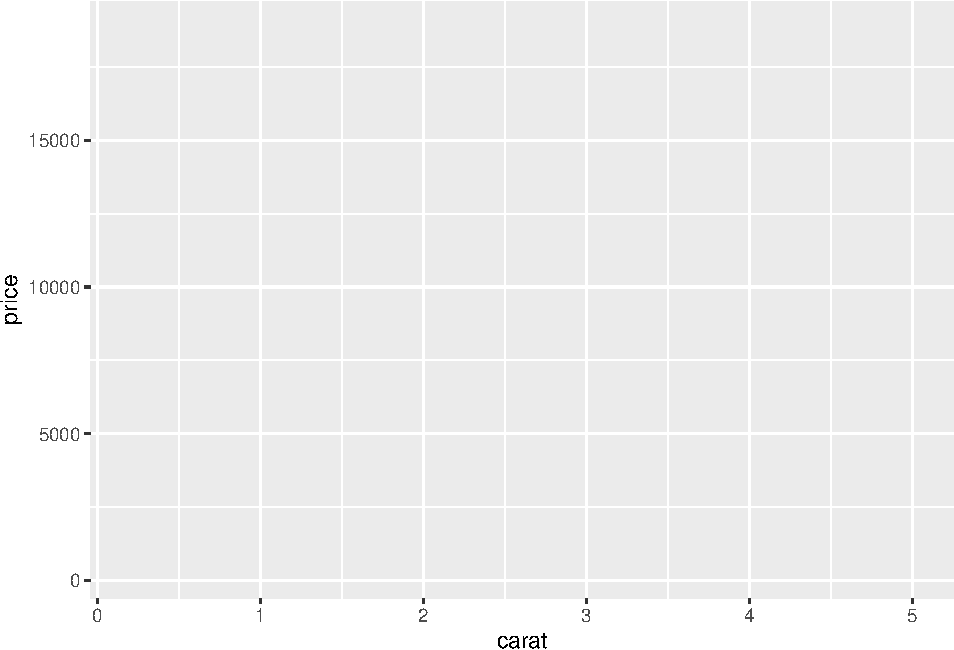
\includegraphics{Introduction-to-R,-Rstudio,-and-ggplot2_files/figure-latex/unnamed-chunk-4-1.pdf}

\begin{Shaded}
\begin{Highlighting}[]
\CommentTok{# geom_points() adds a new layer to a plot by drawing points to produce a scatter plot }
\KeywordTok{ggplot}\NormalTok{(}\DataTypeTok{data =} \NormalTok{diamonds, }\KeywordTok{aes}\NormalTok{(}\DataTypeTok{x =} \NormalTok{carat, }\DataTypeTok{y =} \NormalTok{price)) +}\StringTok{ }\KeywordTok{geom_point}\NormalTok{()}
\end{Highlighting}
\end{Shaded}

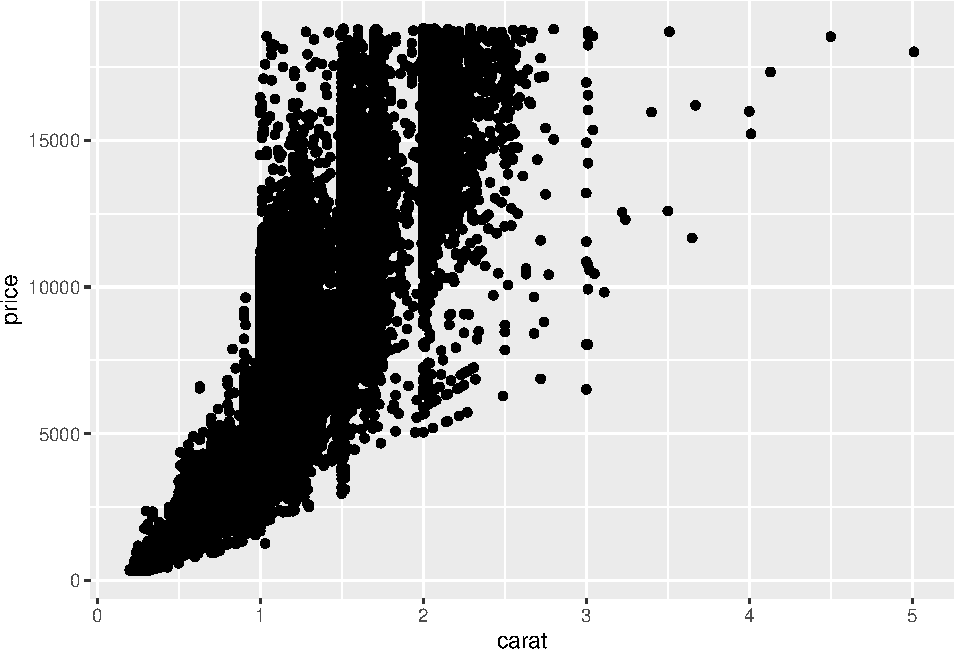
\includegraphics{Introduction-to-R,-Rstudio,-and-ggplot2_files/figure-latex/unnamed-chunk-5-1.pdf}

\begin{Shaded}
\begin{Highlighting}[]
\CommentTok{# geom_smooth() adds an additional layer to the plot by drawing a smoothed line to capture the trend in the scatterplot}
\KeywordTok{ggplot}\NormalTok{(}\DataTypeTok{data =} \NormalTok{diamonds, }\KeywordTok{aes}\NormalTok{(}\DataTypeTok{x =} \NormalTok{carat, }\DataTypeTok{y =} \NormalTok{price)) +}\StringTok{ }\KeywordTok{geom_point}\NormalTok{() +}\StringTok{ }\KeywordTok{geom_smooth}\NormalTok{()}
\end{Highlighting}
\end{Shaded}

\begin{verbatim}
## `geom_smooth()` using method = 'gam' and formula 'y ~ s(x, bs = "cs")'
\end{verbatim}

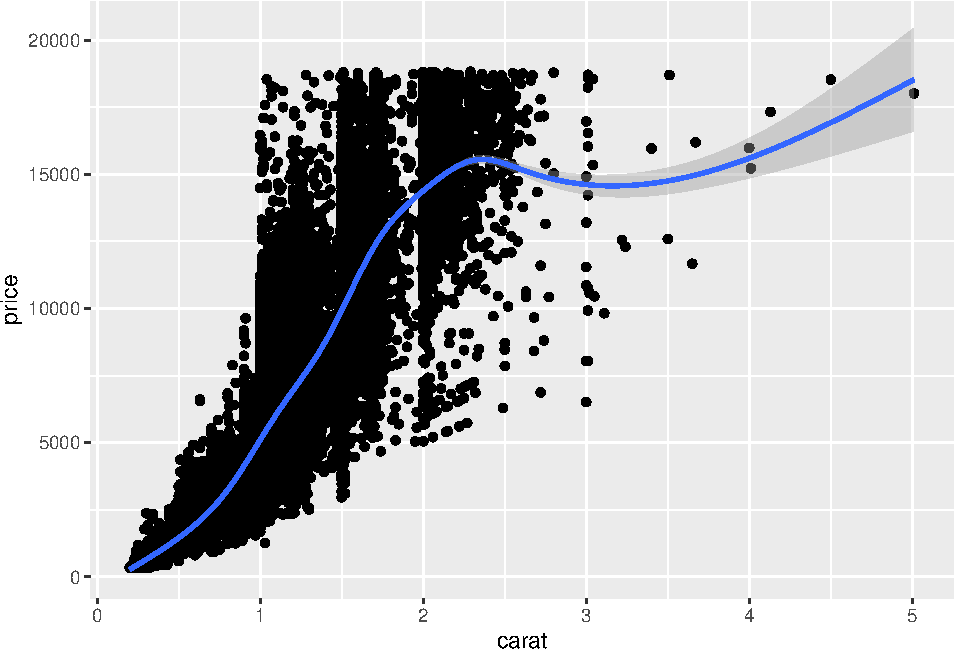
\includegraphics{Introduction-to-R,-Rstudio,-and-ggplot2_files/figure-latex/unnamed-chunk-6-1.pdf}

\section{Exercise}\label{exercise}

\begin{itemize}
\item
  typing \texttt{mtcars} in your console will display the content of the
  \texttt{mtcars} dataset. How can we display the help document for the
  \texttt{mtcars} data?
\item
  type \texttt{head(mtcars)}. What did \texttt{head()} do? Check the
  help document of \texttt{head()} (\texttt{mtcar} is a dataframe in
  base R, whereas the \texttt{diamonds} is a tibble in
  \texttt{tidyverse}).
\item
  Using the \texttt{mtcars} data, plot the scatter plot between
  \texttt{mpg} (miles per gallon: y axis) and \texttt{disp}
  (displacement: x axis) with a smoothed line.
\end{itemize}

\section{Aesthetic mappings}\label{aesthetic-mappings}

\begin{itemize}
\item
  ``A set of aesthetic mappings describe how \textbf{variables in the
  data} are mapped to \textbf{aesthetic properties} of the layer''
  \citep{ggplot2}
\item
  ``To describe the way that \textbf{variables in the data} are mapped
  to \textbf{things that we can perceive on the plot (the
  ``aesthetics'')}, we use the \texttt{aes} function. The \texttt{aes}
  function takes a list of aesthetic-variable pairs like these:
  \texttt{aes(x\ =\ weight,\ y\ =\ height,\ colour\ =\ age)}. Here we
  are mapping x-position to \texttt{weight}, y-position to
  \texttt{height} and colour to \texttt{age}. The first two arguments
  can be left without names, in which case they correspond to the x and
  y variables.'' \citep{ggplot2}
\end{itemize}

\begin{Shaded}
\begin{Highlighting}[]
\CommentTok{# color = color maps the variable 'color` in the dataset to the color aesthetics of points to encode further information in the graphic. }
\KeywordTok{ggplot}\NormalTok{(}\DataTypeTok{data =} \NormalTok{diamonds, }\KeywordTok{aes}\NormalTok{(}\DataTypeTok{x =} \NormalTok{carat, }\DataTypeTok{y =} \NormalTok{price, }\DataTypeTok{color =} \NormalTok{color)) +}\StringTok{ }\KeywordTok{geom_point}\NormalTok{()}
\end{Highlighting}
\end{Shaded}

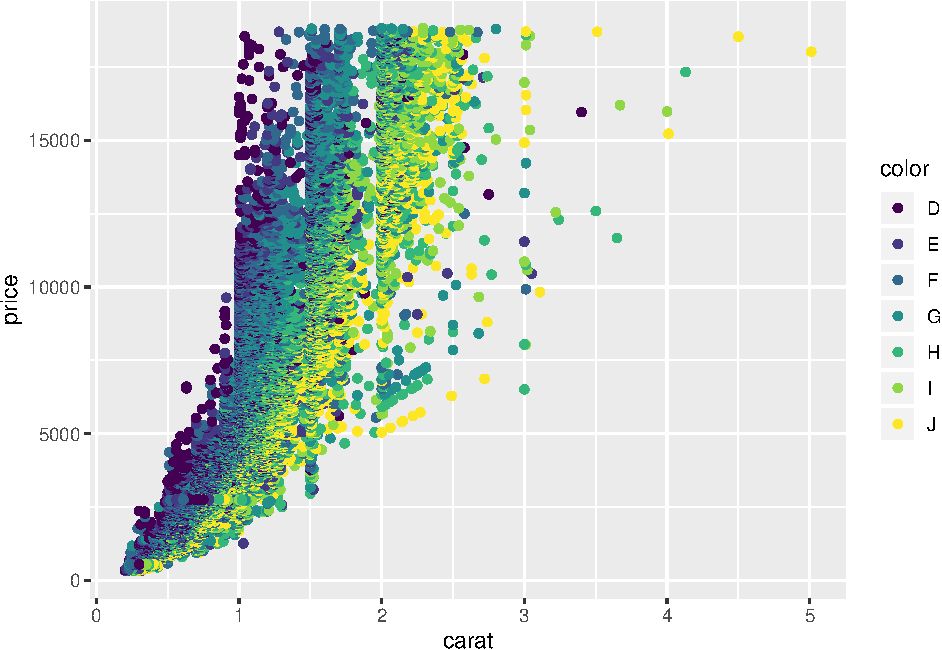
\includegraphics{Introduction-to-R,-Rstudio,-and-ggplot2_files/figure-latex/unnamed-chunk-7-1.pdf}

\begin{Shaded}
\begin{Highlighting}[]
\CommentTok{# shape = cut maps the variable 'cut` in the dataset to the shape aesthetics of points to encode further information in the graphic. }
\CommentTok{# the graphic is not so informative because points are overplotted. Sometimes, facetting may handle overplotting }
\KeywordTok{ggplot}\NormalTok{(}\DataTypeTok{data =} \NormalTok{diamonds, }\KeywordTok{aes}\NormalTok{(}\DataTypeTok{x =} \NormalTok{carat, }\DataTypeTok{y =} \NormalTok{price, }\DataTypeTok{shape =} \NormalTok{cut)) +}\StringTok{ }\KeywordTok{geom_point}\NormalTok{()}
\end{Highlighting}
\end{Shaded}

\begin{verbatim}
## Warning: Using shapes for an ordinal variable is not advised
\end{verbatim}

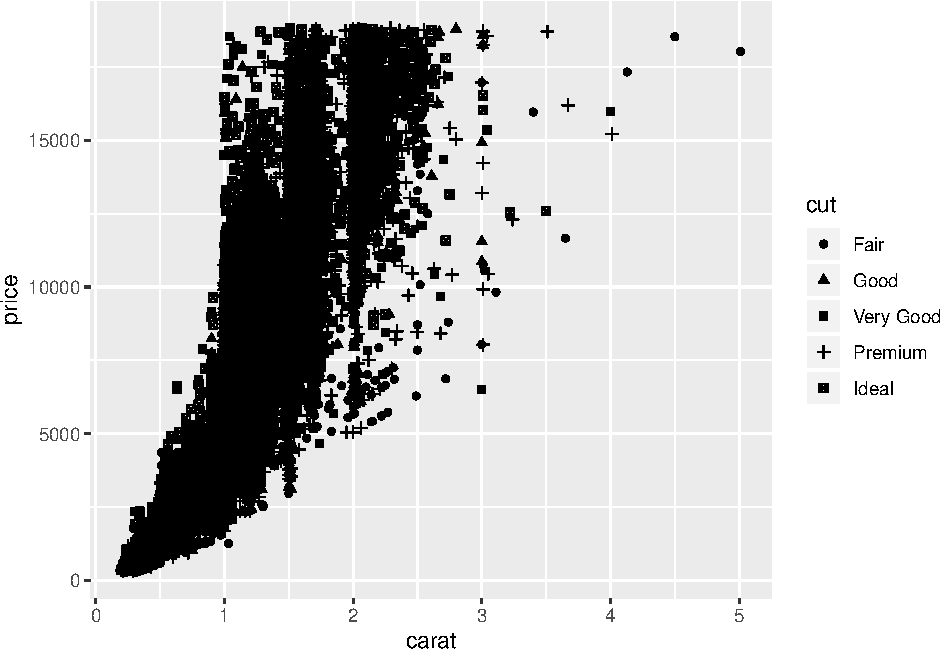
\includegraphics{Introduction-to-R,-Rstudio,-and-ggplot2_files/figure-latex/unnamed-chunk-8-1.pdf}

\begin{Shaded}
\begin{Highlighting}[]
\KeywordTok{ggplot}\NormalTok{(}\DataTypeTok{data =} \NormalTok{diamonds, }\KeywordTok{aes}\NormalTok{(}\DataTypeTok{x =} \NormalTok{carat, }\DataTypeTok{y =} \NormalTok{price)) +}\StringTok{ }\KeywordTok{geom_point}\NormalTok{(}\DataTypeTok{color =} \StringTok{"blue"}\NormalTok{)}
\end{Highlighting}
\end{Shaded}

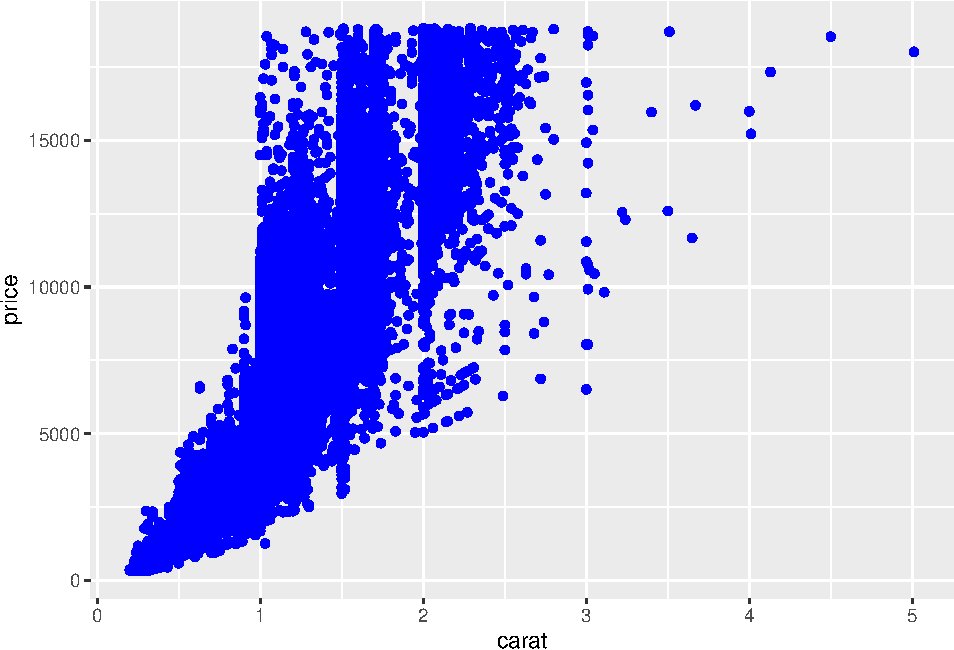
\includegraphics{Introduction-to-R,-Rstudio,-and-ggplot2_files/figure-latex/unnamed-chunk-9-1.pdf}

\section{Exercise}\label{exercise-1}

\begin{itemize}
\item
  \texttt{mpg} is similar to \texttt{mtcars} but is a built-in tibble in
  \texttt{ggplot2}. 1) Plot \texttt{hwy} (mile per gallon: y axis)
  against \texttt{displ} (engine displancement: x axis), 2) Given the
  plot from 1), map the \texttt{class} variable to color, shape, alpha,
  and size aesthetics.
\item
  Explain what happens.
\end{itemize}

\begin{Shaded}
\begin{Highlighting}[]
\KeywordTok{ggplot}\NormalTok{(}\DataTypeTok{data =} \NormalTok{mpg, }\DataTypeTok{mapping =} \KeywordTok{aes}\NormalTok{(}\DataTypeTok{x =} \NormalTok{displ, }\DataTypeTok{y =} \NormalTok{hwy, }\DataTypeTok{color=}\NormalTok{drv)) +}\StringTok{ }\KeywordTok{geom_point}\NormalTok{() +}\StringTok{ }\KeywordTok{geom_smooth}\NormalTok{(}\DataTypeTok{method=}\StringTok{"lm"}\NormalTok{)}
\end{Highlighting}
\end{Shaded}

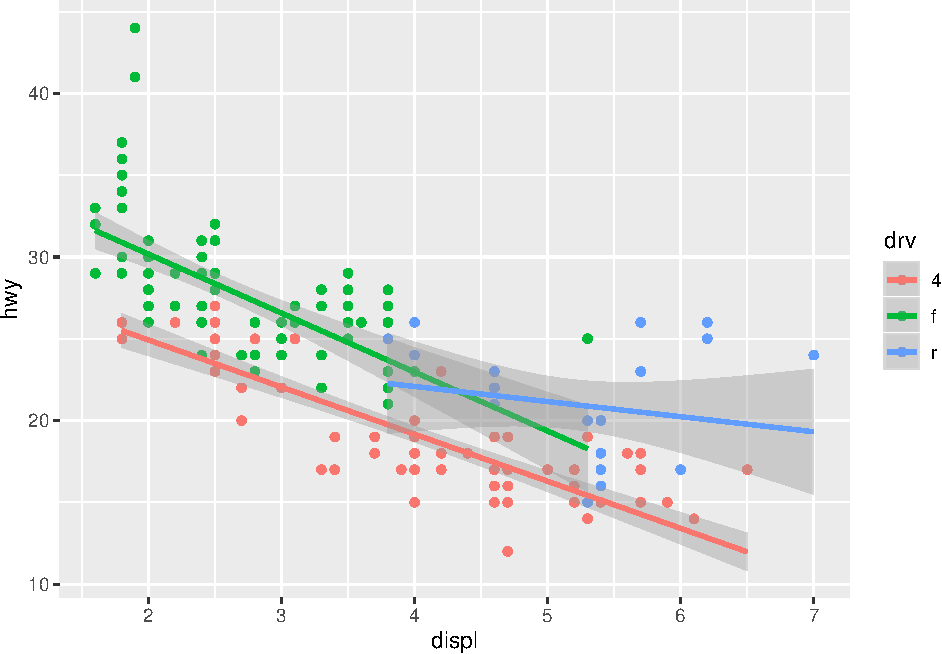
\includegraphics{Introduction-to-R,-Rstudio,-and-ggplot2_files/figure-latex/unnamed-chunk-10-1.pdf}

\begin{itemize}
\tightlist
\item
  This is what happens when mapping \texttt{hyw}, \texttt{displ}, and
  \texttt{cyl} to \texttt{x}, \texttt{y}, and \texttt{color} aesthetics.
  R creates a new dataset that contains all the data to be displayed on
  the plot.
\end{itemize}

\begin{longtable}[]{@{}lll@{}}
\toprule
x & y & color\tabularnewline
\midrule
\endhead
1.8 & 29 & 4\tabularnewline
1.8 & 29 & 4\tabularnewline
2.0 & 31 & 4\tabularnewline
2.0 & 30 & 4\tabularnewline
2.8 & 26 & 6\tabularnewline
2.8 & 26 & 6\tabularnewline
3.1 & 27 & 6\tabularnewline
1.8 & 26 & 4\tabularnewline
1.8 & 25 & 4\tabularnewline
2.0 & 28 & 4\tabularnewline
\bottomrule
\end{longtable}

\section{Scales}\label{scales}

\begin{itemize}
\item
  In the previous table, computers don't know how to display colors
  based on 4, 6, \ldots{} Computers need a a hexadecimal code for colors
  such as \texttt{FF6C91}. The mapping from the data to the final values
  that computers can use to display aesthetics is called a scale.
\item
  ``The scales map values in the data space to values in an aesthetic
  space, whether it be colour, or size, or shape. Scales draw a legend
  or axes, which provide an inverse mapping to make it possible to read
  the original data values from the graph.'' \citep{ggplot2}
\item
  \texttt{scale\_x\_continuous()} and \texttt{scale\_y\_continuous()}
  are the default scales for continuous x and y aesthetics:
  \url{https://ggplot2.tidyverse.org/reference/scale_continuous.html}.
\end{itemize}

\begin{Shaded}
\begin{Highlighting}[]
\NormalTok{p1 <-}\StringTok{ }\KeywordTok{ggplot}\NormalTok{(mpg, }\KeywordTok{aes}\NormalTok{(displ, hwy)) +}\StringTok{ }\KeywordTok{geom_point}\NormalTok{()}
\NormalTok{p1}
\end{Highlighting}
\end{Shaded}

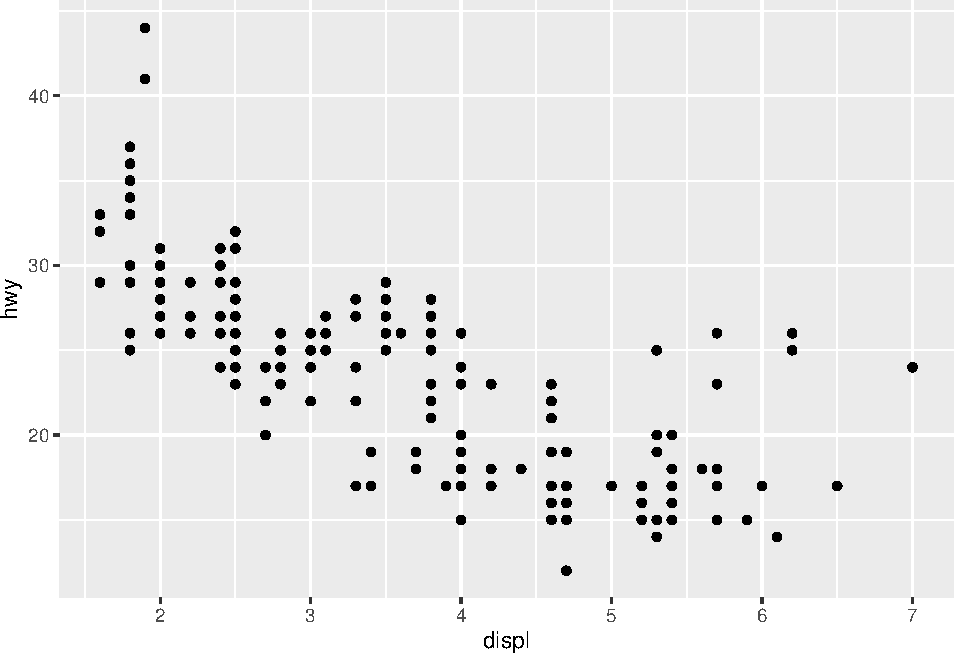
\includegraphics{Introduction-to-R,-Rstudio,-and-ggplot2_files/figure-latex/unnamed-chunk-11-1.pdf}

\begin{Shaded}
\begin{Highlighting}[]
\CommentTok{# change the axis labels}
\NormalTok{p1 +}\StringTok{ }\KeywordTok{scale_x_continuous}\NormalTok{(}\StringTok{"Engine displacement (L)"}\NormalTok{) +}
\StringTok{  }\KeywordTok{scale_y_continuous}\NormalTok{(}\StringTok{"Highway MPG"}\NormalTok{)}
\end{Highlighting}
\end{Shaded}

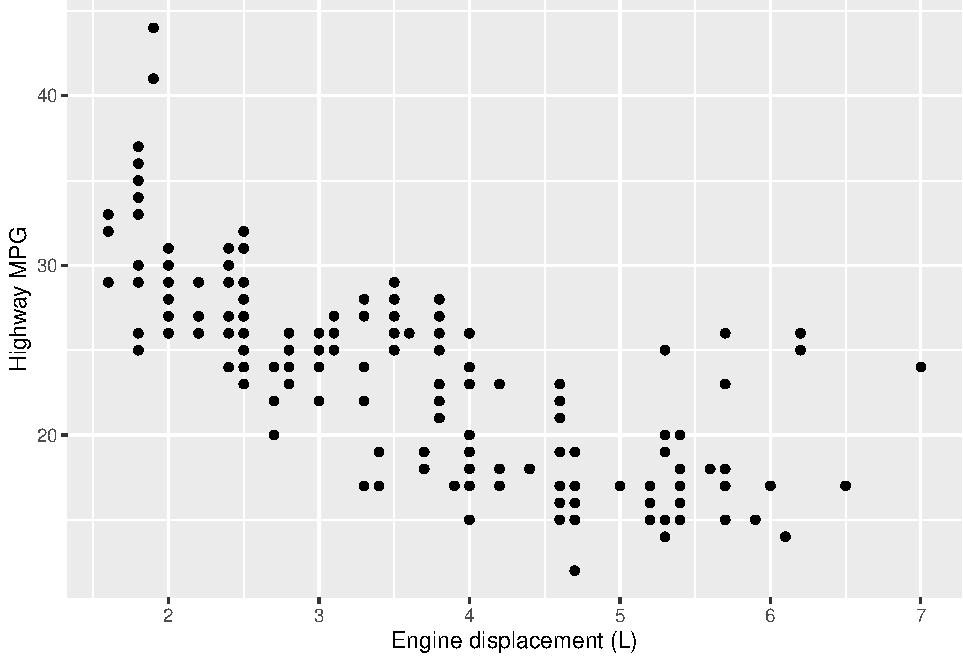
\includegraphics{Introduction-to-R,-Rstudio,-and-ggplot2_files/figure-latex/unnamed-chunk-12-1.pdf}

\begin{Shaded}
\begin{Highlighting}[]
\CommentTok{# also use the short-cut labs()}
\NormalTok{p1 +}\StringTok{ }\KeywordTok{labs}\NormalTok{(}\DataTypeTok{x =} \StringTok{"Engine displacement (L)"}\NormalTok{, }\DataTypeTok{y =} \StringTok{"Highway MPG"}\NormalTok{)}
\end{Highlighting}
\end{Shaded}

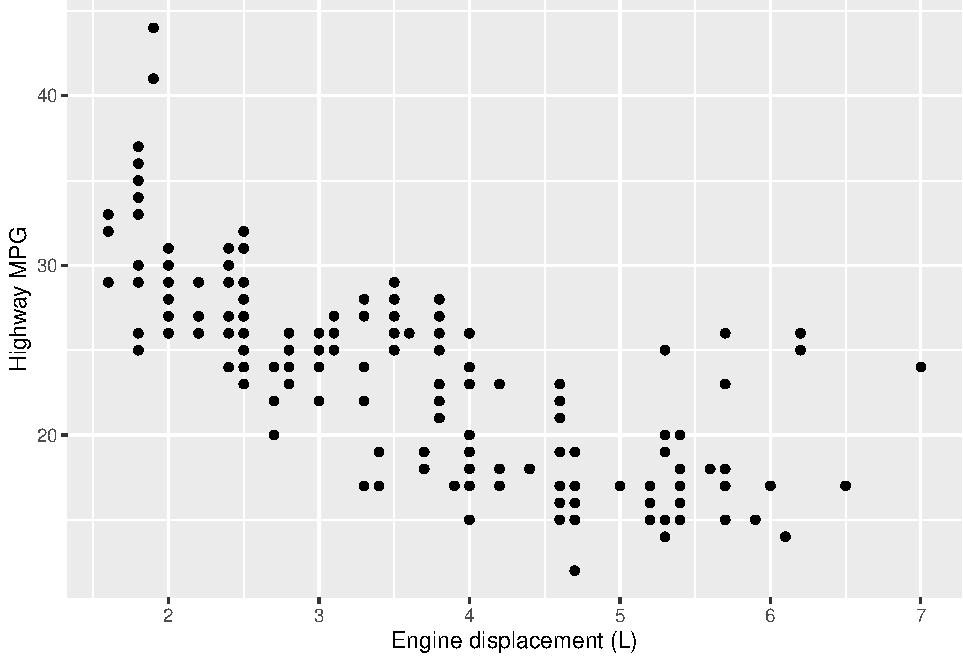
\includegraphics{Introduction-to-R,-Rstudio,-and-ggplot2_files/figure-latex/unnamed-chunk-13-1.pdf}

\begin{Shaded}
\begin{Highlighting}[]
\CommentTok{# modify the axis limits}
\NormalTok{p1 +}\StringTok{ }\KeywordTok{scale_x_continuous}\NormalTok{(}\DataTypeTok{limits =} \KeywordTok{c}\NormalTok{(}\DecValTok{2}\NormalTok{, }\DecValTok{6}\NormalTok{))}
\end{Highlighting}
\end{Shaded}

\begin{verbatim}
## Warning: Removed 27 rows containing missing values (geom_point).
\end{verbatim}

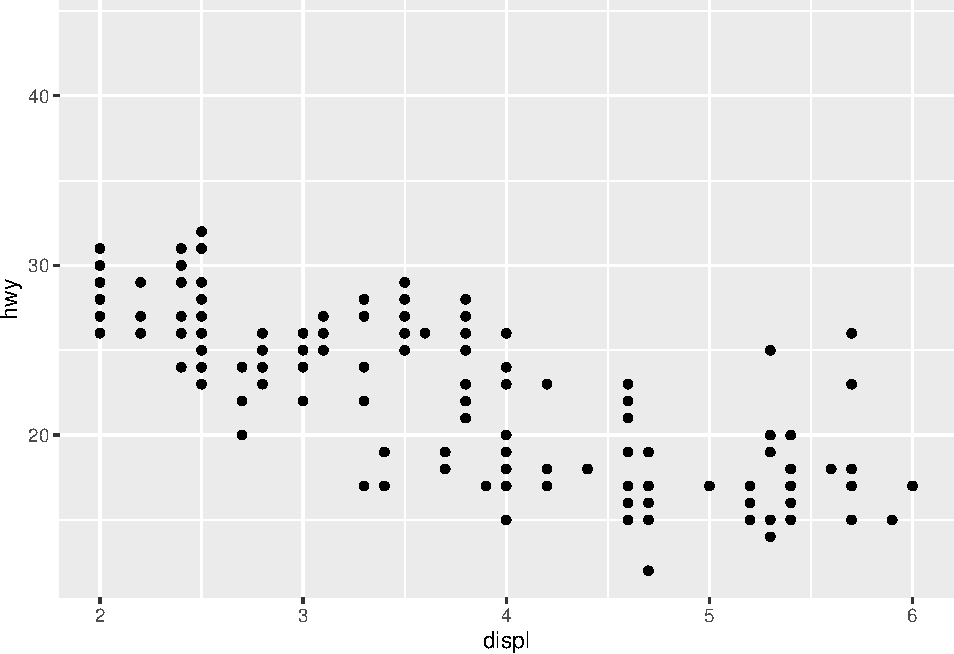
\includegraphics{Introduction-to-R,-Rstudio,-and-ggplot2_files/figure-latex/unnamed-chunk-14-1.pdf}

\begin{Shaded}
\begin{Highlighting}[]
\CommentTok{# use the short hand functions `xlim()` and `ylim()`}
\NormalTok{p1 +}\StringTok{ }\KeywordTok{xlim}\NormalTok{(}\DecValTok{2}\NormalTok{, }\DecValTok{6}\NormalTok{)}
\end{Highlighting}
\end{Shaded}

\begin{verbatim}
## Warning: Removed 27 rows containing missing values (geom_point).
\end{verbatim}

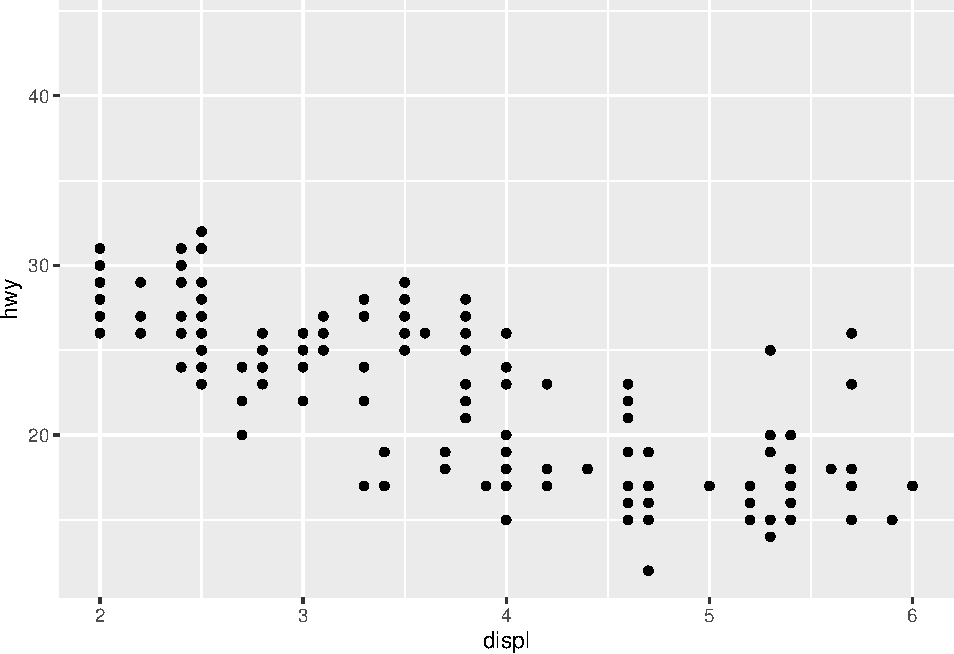
\includegraphics{Introduction-to-R,-Rstudio,-and-ggplot2_files/figure-latex/unnamed-chunk-15-1.pdf}

\begin{Shaded}
\begin{Highlighting}[]
\CommentTok{#  choose where the ticks appear}
\NormalTok{p1 +}\StringTok{ }\KeywordTok{scale_x_continuous}\NormalTok{(}\DataTypeTok{breaks =} \KeywordTok{c}\NormalTok{(}\DecValTok{2}\NormalTok{, }\DecValTok{4}\NormalTok{, }\DecValTok{6}\NormalTok{))}
\end{Highlighting}
\end{Shaded}

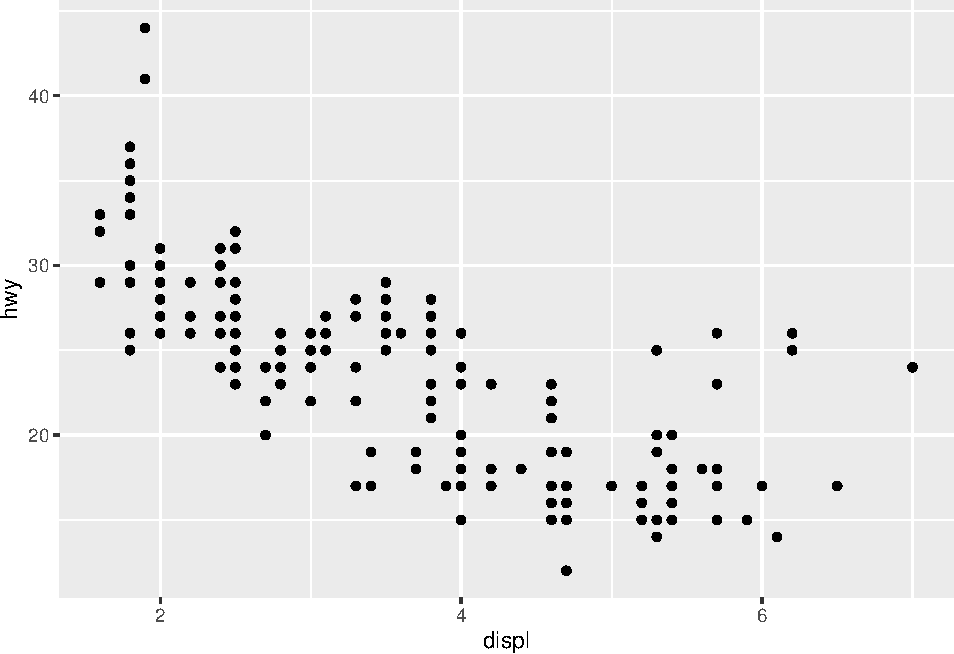
\includegraphics{Introduction-to-R,-Rstudio,-and-ggplot2_files/figure-latex/unnamed-chunk-16-1.pdf}

\begin{Shaded}
\begin{Highlighting}[]
\CommentTok{#  choose your own labels}
\NormalTok{p1 +}\StringTok{ }\KeywordTok{scale_x_continuous}\NormalTok{(}\DataTypeTok{breaks =} \KeywordTok{c}\NormalTok{(}\DecValTok{2}\NormalTok{, }\DecValTok{4}\NormalTok{, }\DecValTok{6}\NormalTok{), }\DataTypeTok{label =} \KeywordTok{c}\NormalTok{(}\StringTok{"two"}\NormalTok{, }\StringTok{"four"}\NormalTok{, }\StringTok{"six"}\NormalTok{))}
\end{Highlighting}
\end{Shaded}

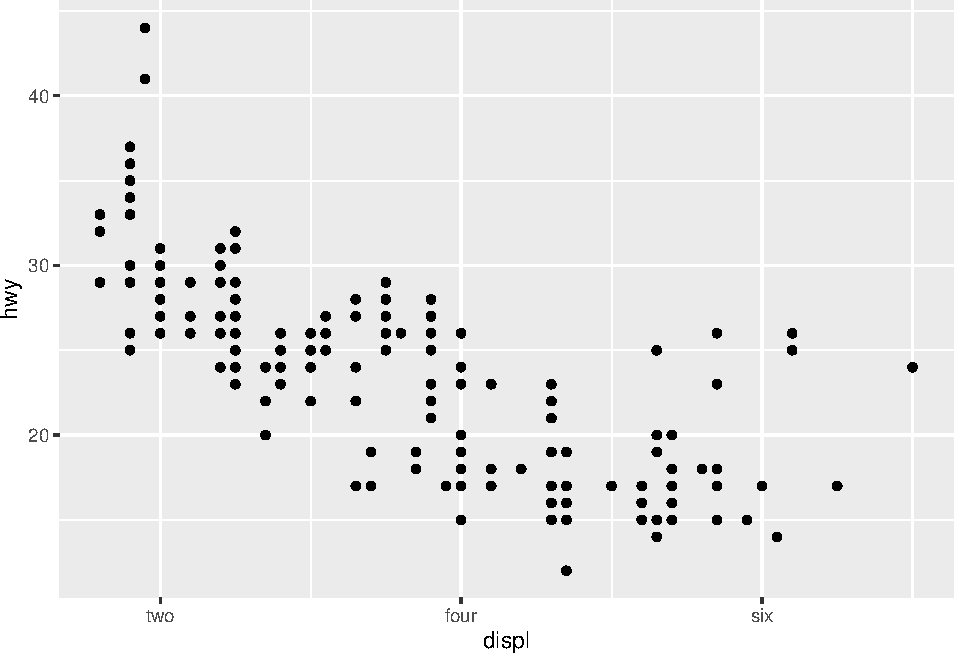
\includegraphics{Introduction-to-R,-Rstudio,-and-ggplot2_files/figure-latex/unnamed-chunk-17-1.pdf}

\begin{Shaded}
\begin{Highlighting}[]
\KeywordTok{ggplot}\NormalTok{(}\DataTypeTok{data =} \NormalTok{mpg, }\DataTypeTok{mapping =} \KeywordTok{aes}\NormalTok{(}\DataTypeTok{x =} \NormalTok{displ, }\DataTypeTok{y =} \NormalTok{hwy, }\DataTypeTok{color=}\NormalTok{drv)) +}\StringTok{ }\KeywordTok{geom_point}\NormalTok{() +}\StringTok{ }\KeywordTok{geom_smooth}\NormalTok{(}\DataTypeTok{method=}\StringTok{"lm"}\NormalTok{) +}\StringTok{ }\KeywordTok{labs}\NormalTok{(}\DataTypeTok{title =}\StringTok{"MPG vs Engine size"}\NormalTok{, }\DataTypeTok{x =} \StringTok{"Engine size"}\NormalTok{, }\DataTypeTok{y =} \StringTok{"MPG"}\NormalTok{)}
\end{Highlighting}
\end{Shaded}

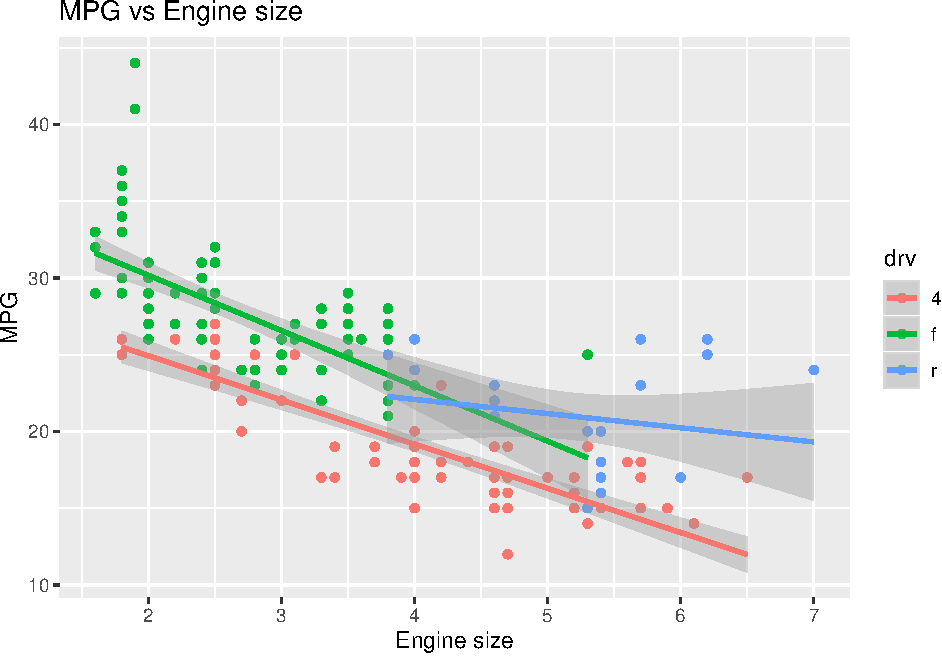
\includegraphics{Introduction-to-R,-Rstudio,-and-ggplot2_files/figure-latex/unnamed-chunk-18-1.pdf}

\section{\texorpdfstring{Statistical transformations (\textbf{stats} for
short)}{Statistical transformations (stats for short)}}\label{statistical-transformations-stats-for-short}

\begin{Shaded}
\begin{Highlighting}[]
\CommentTok{# historam shows the distribution of a single variable. }
\CommentTok{# where does count come from? }
\KeywordTok{ggplot}\NormalTok{(}\DataTypeTok{data =} \NormalTok{diamonds, }\KeywordTok{aes}\NormalTok{(}\DataTypeTok{x =} \NormalTok{carat)) +}\StringTok{ }\KeywordTok{geom_histogram}\NormalTok{()}
\end{Highlighting}
\end{Shaded}

\begin{verbatim}
## `stat_bin()` using `bins = 30`. Pick better value with `binwidth`.
\end{verbatim}

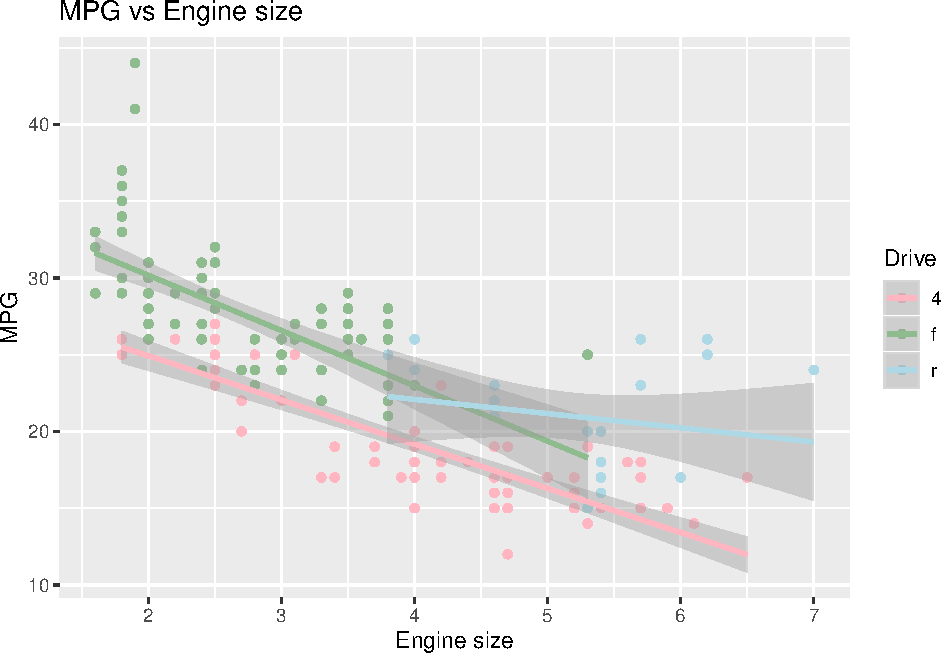
\includegraphics{Introduction-to-R,-Rstudio,-and-ggplot2_files/figure-latex/unnamed-chunk-19-1.pdf}

\begin{itemize}
\item
  ``Statistical transformations, \textbf{stats} for short, summarise
  data in many useful ways. For example, binning and counting
  observations to create a histogram, or summarising a 2d relationship
  with a linear model. Stats are optional, but very useful.''
  \citep{ggplot2}
\item
  How \texttt{geom\_histogram()} works?

  \begin{itemize}
  \tightlist
  \item
    ``A stat takes a dataset as input and returns a dataset as output,
    and so a stat can add new variables to the original dataset. It is
    possible to map aesthetics to these new variables. For example,
    \texttt{stat\_bin}, the statistic used to make histograms, produces
    the following variables:

    \begin{itemize}
    \tightlist
    \item
      \texttt{count}, the number of observations in each bin
    \item
      \texttt{density}, the density of observations in each bin
      (percentage of total / bar width)
    \item
      \texttt{x}, the centre of the bin" \citep{ggplot2}
    \end{itemize}
  \item
    ``These generated variables can be used instead of the variables
    present in the original dataset. For example, the default histogram
    geom assigns the height of the bars to the number of observations
    (\texttt{count}), but if you'd prefer a more traditional histogram,
    you can use the density (\texttt{density}). The following example
    shows a density histogram of carat from the diamonds dataset.''
    \citep{ggplot2}
  \end{itemize}
\end{itemize}

\begin{Shaded}
\begin{Highlighting}[]
\CommentTok{# The names of generated variables must be surrounded with ..}
 \KeywordTok{ggplot}\NormalTok{(diamonds, }\KeywordTok{aes}\NormalTok{(carat)) +}\StringTok{ }\KeywordTok{geom_histogram}\NormalTok{(}\KeywordTok{aes}\NormalTok{(}\DataTypeTok{y =} \NormalTok{..density..), }\DataTypeTok{binwidth =} \FloatTok{0.1}\NormalTok{)}
\end{Highlighting}
\end{Shaded}

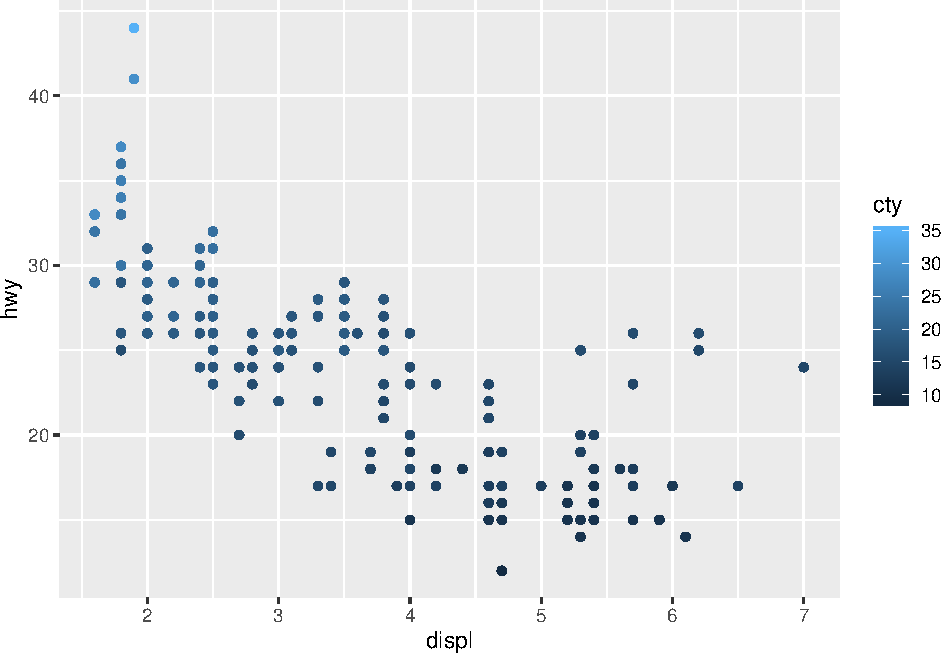
\includegraphics{Introduction-to-R,-Rstudio,-and-ggplot2_files/figure-latex/unnamed-chunk-20-1.pdf}

\begin{itemize}
\item
  Every \textbf{geom} has a default \textbf{stats}.
\item
  Position adjustments

  \begin{itemize}
  \tightlist
  \item
    Position adjustments determine how to arrange \textbf{geoms} that
    would otherwise occupy the same space.
  \end{itemize}
\end{itemize}

\begin{Shaded}
\begin{Highlighting}[]
\CommentTok{# The discrete analogue of histogram is the bar plot}
\NormalTok{s <-}\StringTok{ }\KeywordTok{ggplot}\NormalTok{(mpg, }\KeywordTok{aes}\NormalTok{(fl, }\DataTypeTok{fill =} \NormalTok{drv))}
\end{Highlighting}
\end{Shaded}

\begin{Shaded}
\begin{Highlighting}[]
\NormalTok{s +}\StringTok{ }\KeywordTok{geom_bar}\NormalTok{()}
\end{Highlighting}
\end{Shaded}

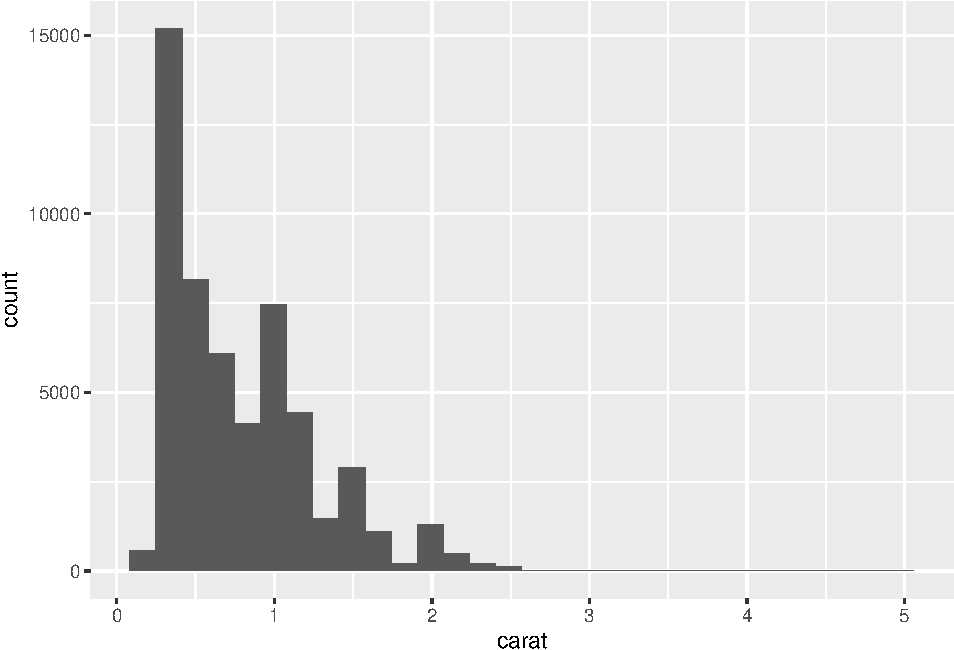
\includegraphics{Introduction-to-R,-Rstudio,-and-ggplot2_files/figure-latex/unnamed-chunk-22-1.pdf}

\begin{Shaded}
\begin{Highlighting}[]
\CommentTok{# Stack elements on top of one another}
\NormalTok{s +}\StringTok{ }\KeywordTok{geom_bar}\NormalTok{(}\DataTypeTok{position =} \StringTok{"stack"}\NormalTok{)}
\end{Highlighting}
\end{Shaded}

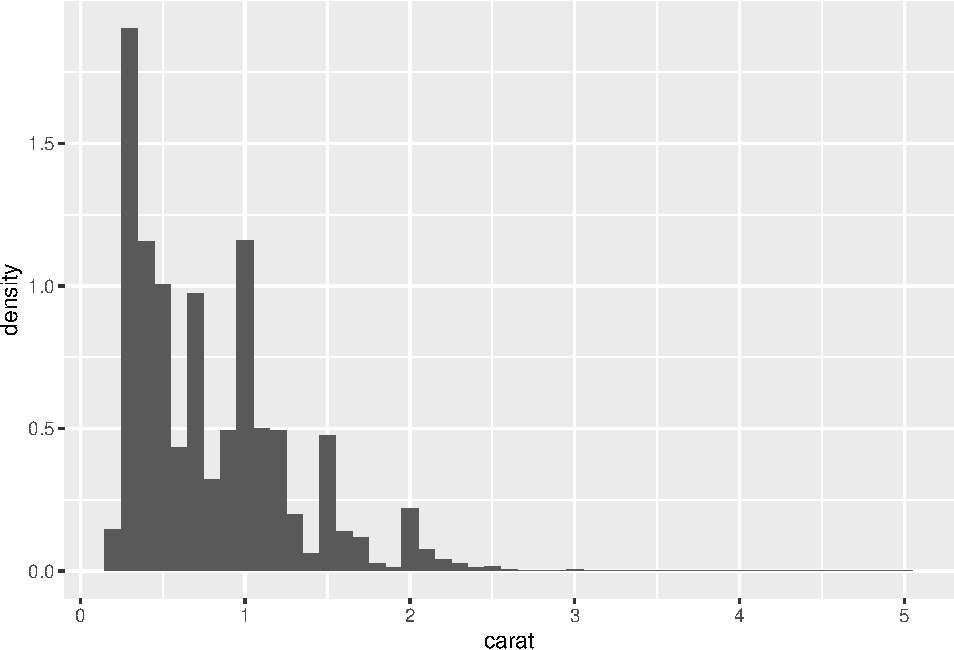
\includegraphics{Introduction-to-R,-Rstudio,-and-ggplot2_files/figure-latex/unnamed-chunk-23-1.pdf}

\begin{Shaded}
\begin{Highlighting}[]
\CommentTok{# Arrange elements side by side}
\NormalTok{s +}\StringTok{ }\KeywordTok{geom_bar}\NormalTok{(}\DataTypeTok{position =} \StringTok{"dodge"}\NormalTok{)}
\end{Highlighting}
\end{Shaded}

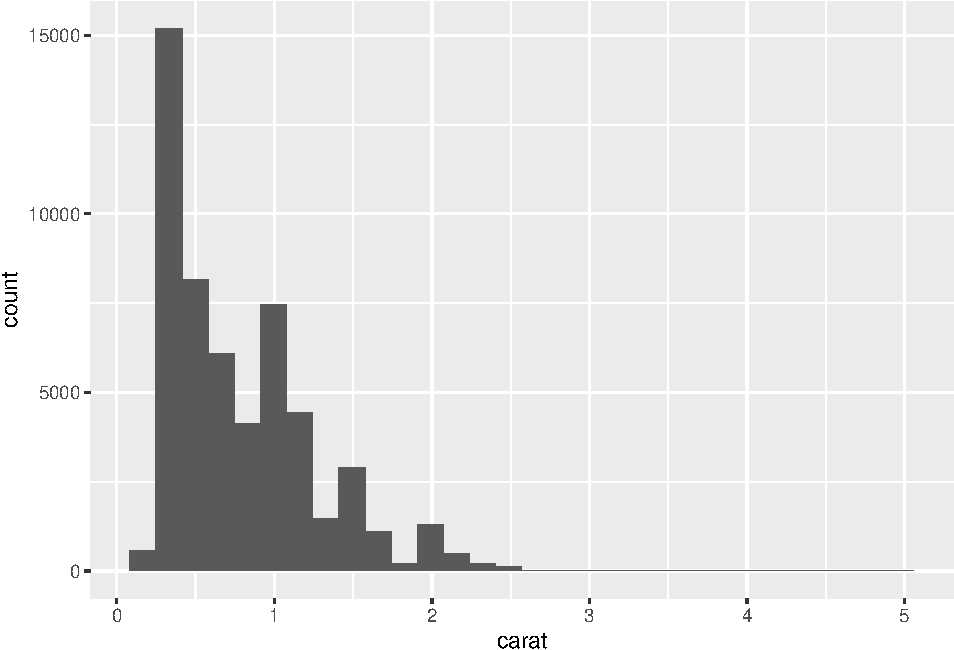
\includegraphics{Introduction-to-R,-Rstudio,-and-ggplot2_files/figure-latex/unnamed-chunk-24-1.pdf}

\begin{Shaded}
\begin{Highlighting}[]
\CommentTok{# Stack elements on top of one another,normalize height}
\NormalTok{s +}\StringTok{ }\KeywordTok{geom_bar}\NormalTok{(}\DataTypeTok{position =} \StringTok{"fill"}\NormalTok{)}
\end{Highlighting}
\end{Shaded}

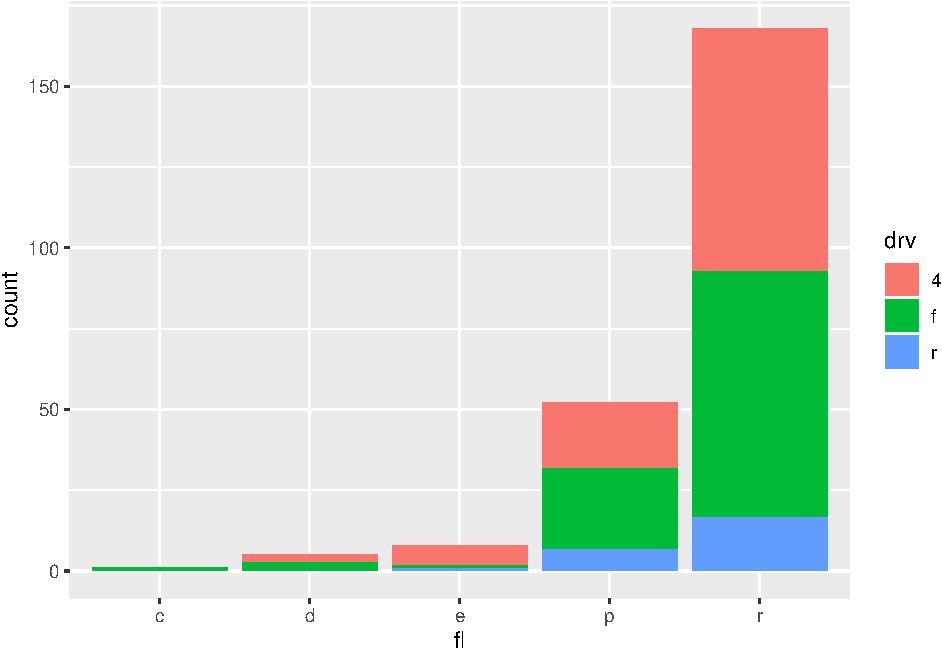
\includegraphics{Introduction-to-R,-Rstudio,-and-ggplot2_files/figure-latex/unnamed-chunk-25-1.pdf}

\section{A faceting}\label{a-faceting}

\begin{itemize}
\item
  ``A faceting specification describes how to break up the data into
  \textbf{subsets} and how to display those subsets as \textbf{small
  multiples}. This is also known as \textbf{conditioning} or
  latticing/trellising.'' \citep{ggplot2}
\item
  ``There are two types of faceting provided by ggplot2:
  \texttt{facet\_grid} and \texttt{facet\_wrap}. Facet grid produces a
  2d grid of panels defined by variables which form the rows and
  columns, while facet wrap produces a 1d ribbon of panels that is
  wrapped into 2d'' \citep{ggplot2}
\end{itemize}

\begin{Shaded}
\begin{Highlighting}[]
\CommentTok{# facet into rows}
\KeywordTok{ggplot}\NormalTok{(}\DataTypeTok{data =} \NormalTok{diamonds, }\KeywordTok{aes}\NormalTok{(}\DataTypeTok{x =} \NormalTok{carat)) +}\StringTok{ }\KeywordTok{geom_histogram}\NormalTok{() +}\StringTok{ }\KeywordTok{facet_grid}\NormalTok{(color ~}\StringTok{ }\NormalTok{.)}
\end{Highlighting}
\end{Shaded}

\begin{verbatim}
## `stat_bin()` using `bins = 30`. Pick better value with `binwidth`.
\end{verbatim}

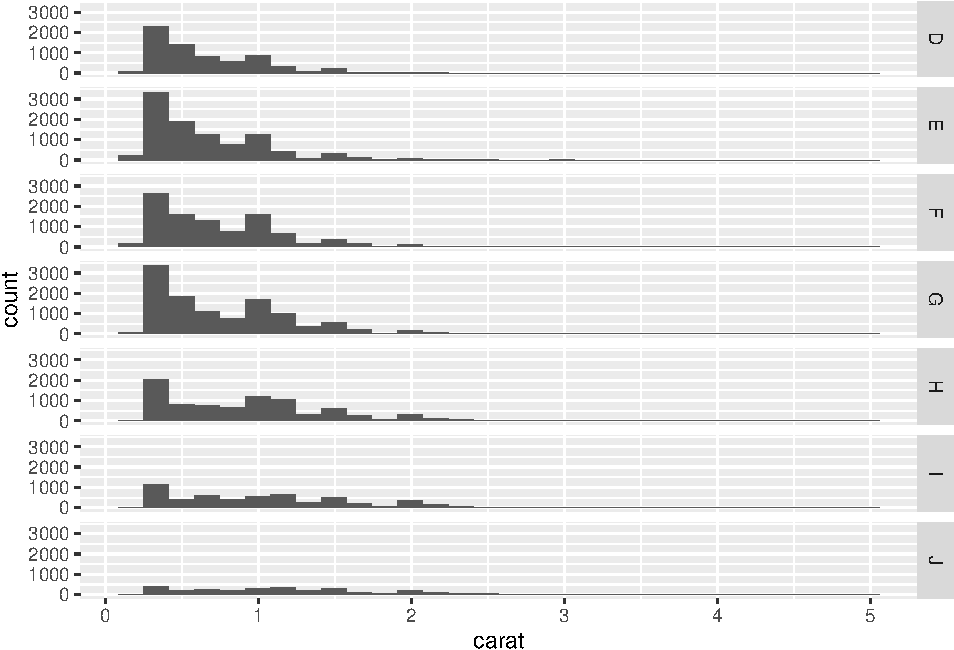
\includegraphics{Introduction-to-R,-Rstudio,-and-ggplot2_files/figure-latex/unnamed-chunk-26-1.pdf}

\begin{Shaded}
\begin{Highlighting}[]
\CommentTok{# facet into columns}
\KeywordTok{ggplot}\NormalTok{(}\DataTypeTok{data =} \NormalTok{diamonds, }\KeywordTok{aes}\NormalTok{(}\DataTypeTok{x =} \NormalTok{carat)) +}\StringTok{ }\KeywordTok{geom_histogram}\NormalTok{() +}\StringTok{ }\KeywordTok{facet_grid}\NormalTok{(. ~}\StringTok{ }\NormalTok{color)}
\end{Highlighting}
\end{Shaded}

\begin{verbatim}
## `stat_bin()` using `bins = 30`. Pick better value with `binwidth`.
\end{verbatim}

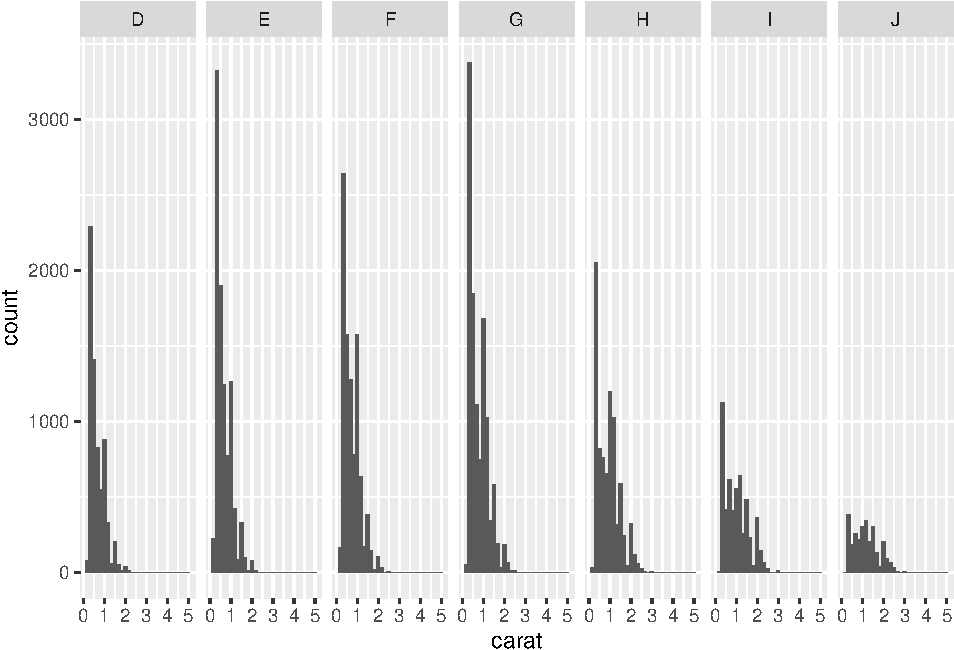
\includegraphics{Introduction-to-R,-Rstudio,-and-ggplot2_files/figure-latex/unnamed-chunk-27-1.pdf}

\section{Exercise}\label{exercise-2}

\begin{itemize}
\item
  Using \texttt{mpg} data, plot \texttt{hwy} (y) vs \texttt{cty} (x).
\item
  facet into rows using \texttt{cyl}.
\item
  facet into columns using \texttt{cyl}.
\item
  facet into rows using \texttt{cyl} and columns using \texttt{year}
\end{itemize}

\section{Grouping}\label{grouping}

\begin{itemize}
\item
  ``In many situations, you want to \textbf{separate your data into
  groups}, but render them in the same way. When looking at the data in
  aggregate you want to be able to distinguish individual subjects, but
  not identify them. This is common in \textbf{longitudinal studies}
  with many subjects, where the plots are often descriptively called
  spaghetti plots.'' \citep{ggplot2}
\item
  \texttt{Oxboys} is a dataset in the \texttt{nlme} package.
  \texttt{Oxboys} includes the height of a selection of boys from
  Oxford, England versus a standardized age.
\end{itemize}

\begin{Shaded}
\begin{Highlighting}[]
\KeywordTok{library}\NormalTok{(nlme)}
\end{Highlighting}
\end{Shaded}

\begin{Shaded}
\begin{Highlighting}[]
\CommentTok{# age = a numeric vector giving the standardized age }
\KeywordTok{head}\NormalTok{(Oxboys)}
\end{Highlighting}
\end{Shaded}

\begin{verbatim}
## Grouped Data: height ~ age | Subject
##   Subject     age height Occasion
## 1       1 -1.0000  140.5        1
## 2       1 -0.7479  143.4        2
## 3       1 -0.4630  144.8        3
## 4       1 -0.1643  147.1        4
## 5       1 -0.0027  147.7        5
## 6       1  0.2466  150.2        6
\end{verbatim}

\begin{Shaded}
\begin{Highlighting}[]
\KeywordTok{ggplot}\NormalTok{(Oxboys, }\KeywordTok{aes}\NormalTok{(age, height)) +}\StringTok{ }\KeywordTok{geom_line}\NormalTok{()}
\end{Highlighting}
\end{Shaded}

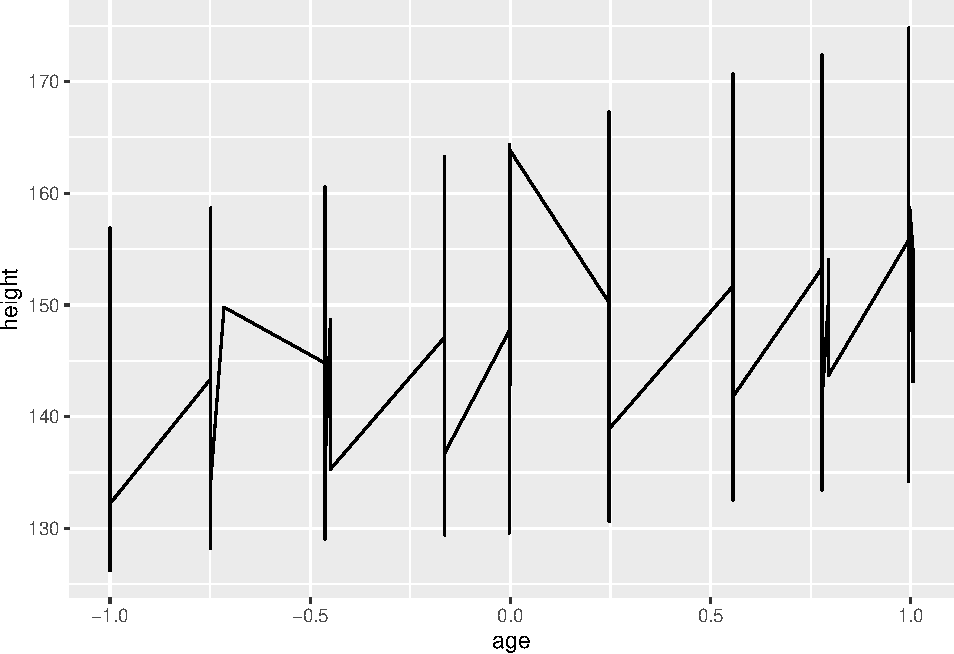
\includegraphics{Introduction-to-R,-Rstudio,-and-ggplot2_files/figure-latex/unnamed-chunk-30-1.pdf}

\begin{Shaded}
\begin{Highlighting}[]
\KeywordTok{ggplot}\NormalTok{(Oxboys, }\KeywordTok{aes}\NormalTok{(age, height, }\DataTypeTok{group =} \NormalTok{Subject)) +}\StringTok{ }\KeywordTok{geom_line}\NormalTok{()}
\end{Highlighting}
\end{Shaded}

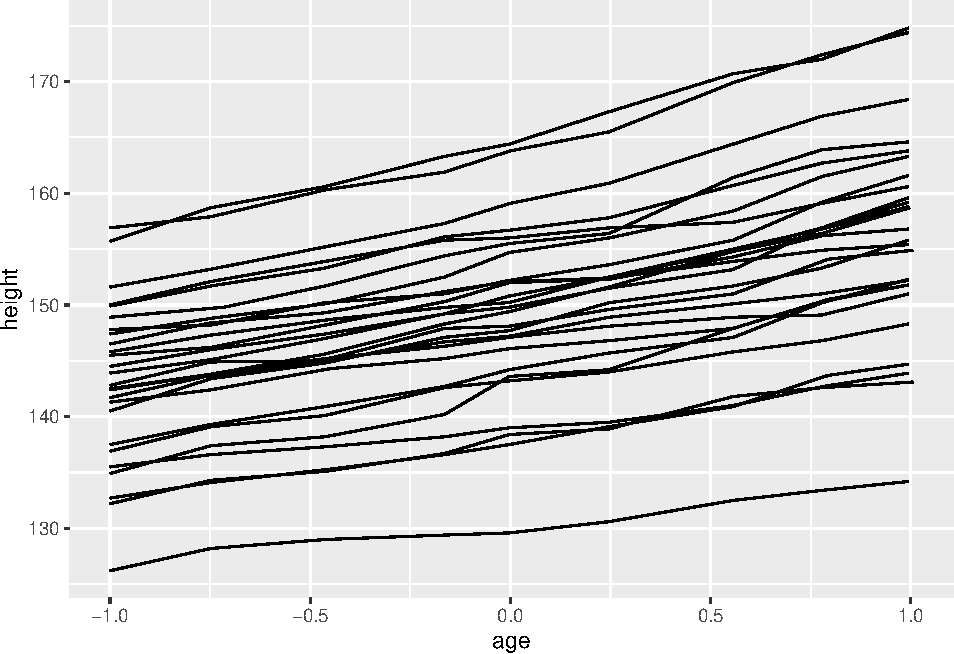
\includegraphics{Introduction-to-R,-Rstudio,-and-ggplot2_files/figure-latex/unnamed-chunk-31-1.pdf}

\begin{Shaded}
\begin{Highlighting}[]
\CommentTok{# In many cases, this is not what we want}
\KeywordTok{ggplot}\NormalTok{(Oxboys, }\KeywordTok{aes}\NormalTok{(age, height, }\DataTypeTok{group =} \NormalTok{Subject)) +}\StringTok{ }\KeywordTok{geom_line}\NormalTok{() +}\StringTok{ }\KeywordTok{geom_smooth}\NormalTok{()}
\end{Highlighting}
\end{Shaded}

\begin{verbatim}
## `geom_smooth()` using method = 'loess' and formula 'y ~ x'
\end{verbatim}

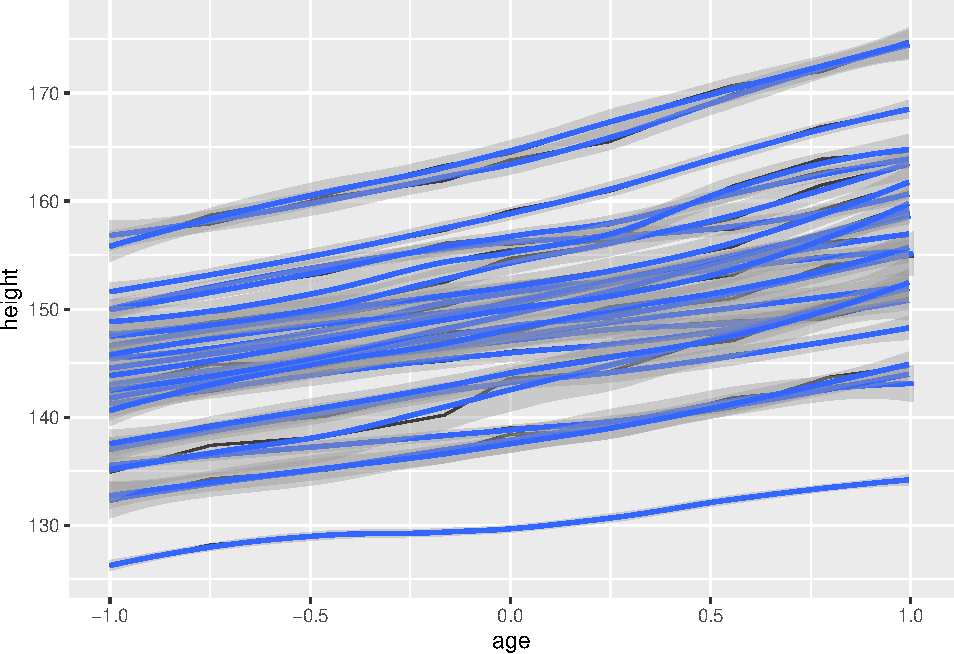
\includegraphics{Introduction-to-R,-Rstudio,-and-ggplot2_files/figure-latex/unnamed-chunk-32-1.pdf}

\begin{Shaded}
\begin{Highlighting}[]
\CommentTok{# group = 1 override the default grouping }
\KeywordTok{ggplot}\NormalTok{(Oxboys, }\KeywordTok{aes}\NormalTok{(age, height, }\DataTypeTok{group =} \NormalTok{Subject)) +}\StringTok{ }\KeywordTok{geom_line}\NormalTok{() +}\StringTok{ }\KeywordTok{geom_smooth}\NormalTok{(}\KeywordTok{aes}\NormalTok{(}\DataTypeTok{group =} \DecValTok{1}\NormalTok{))}
\end{Highlighting}
\end{Shaded}

\begin{verbatim}
## `geom_smooth()` using method = 'loess' and formula 'y ~ x'
\end{verbatim}

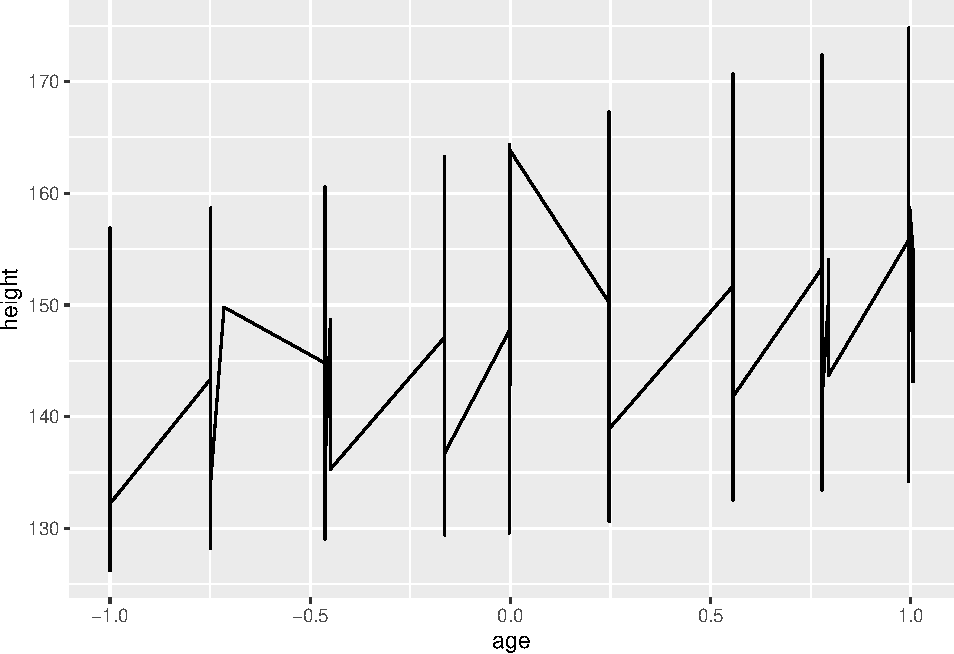
\includegraphics{Introduction-to-R,-Rstudio,-and-ggplot2_files/figure-latex/unnamed-chunk-33-1.pdf}

\begin{Shaded}
\begin{Highlighting}[]
\CommentTok{# facet is also useful for visualizing longitudinal data}
\KeywordTok{ggplot}\NormalTok{(Oxboys, }\KeywordTok{aes}\NormalTok{(age, height)) +}\StringTok{ }\KeywordTok{geom_line}\NormalTok{() +}\StringTok{ }\KeywordTok{facet_wrap}\NormalTok{(~Subject)}
\end{Highlighting}
\end{Shaded}

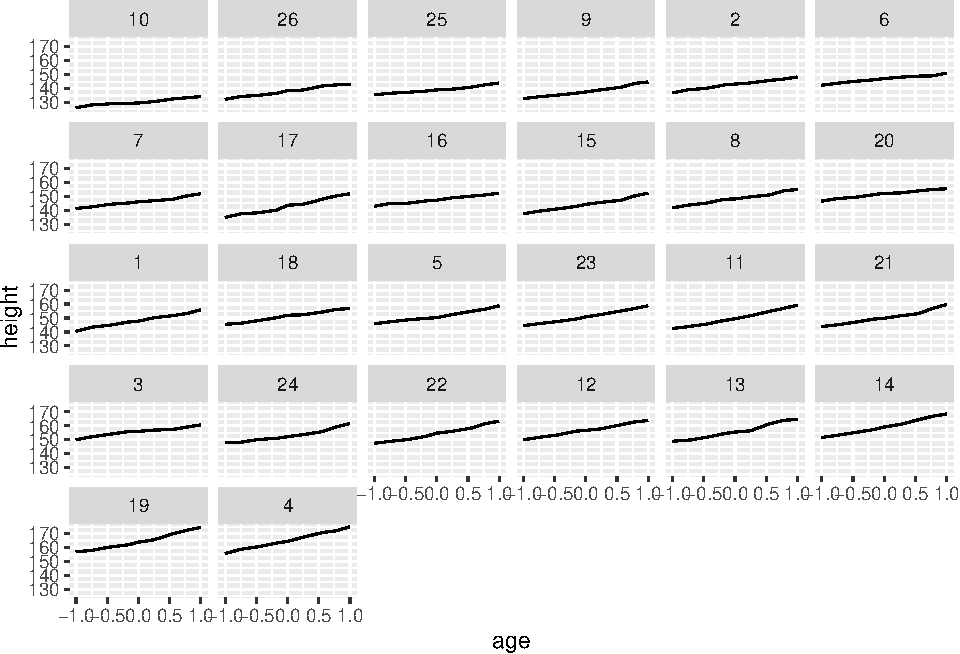
\includegraphics{Introduction-to-R,-Rstudio,-and-ggplot2_files/figure-latex/unnamed-chunk-34-1.pdf}

\section{Themes}\label{themes}

``Themes are a powerful way to \textbf{customize} the non-data
components of your plots: i.e.~titles, labels, fonts, background,
gridlines, and legends.'' More details are available at
\url{https://ggplot2.tidyverse.org/reference/theme.html}

\begin{Shaded}
\begin{Highlighting}[]
\KeywordTok{ggplot}\NormalTok{(mpg, }\KeywordTok{aes}\NormalTok{(}\DataTypeTok{x =} \NormalTok{hwy, }\DataTypeTok{y =} \NormalTok{cty)) +}\StringTok{ }\KeywordTok{geom_point}\NormalTok{() }
\end{Highlighting}
\end{Shaded}

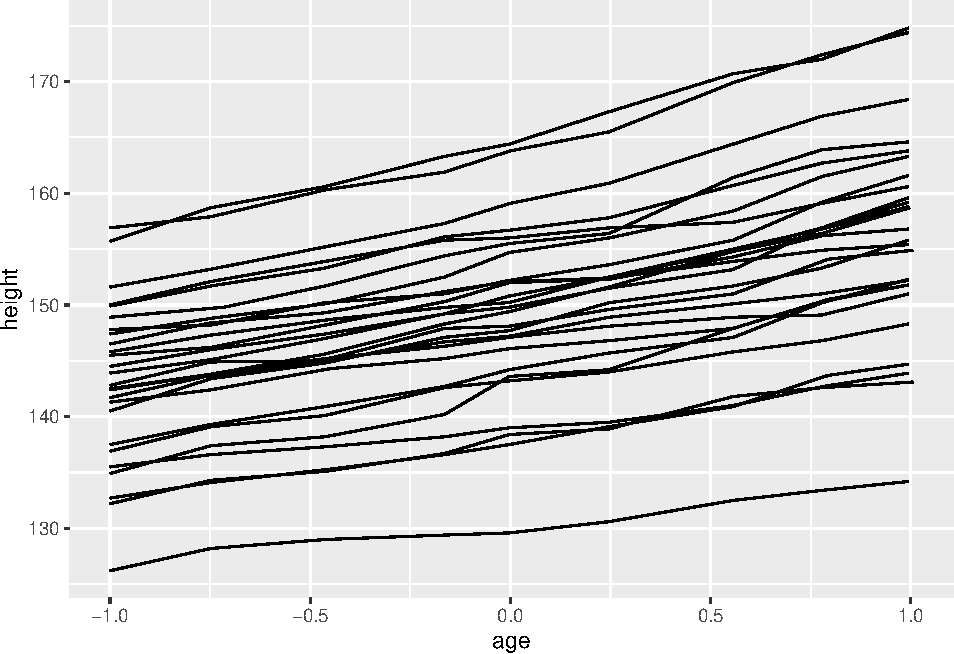
\includegraphics{Introduction-to-R,-Rstudio,-and-ggplot2_files/figure-latex/unnamed-chunk-35-1.pdf}

\begin{Shaded}
\begin{Highlighting}[]
\KeywordTok{ggplot}\NormalTok{(mpg, }\KeywordTok{aes}\NormalTok{(}\DataTypeTok{x =} \NormalTok{hwy, }\DataTypeTok{y =} \NormalTok{cty)) +}\StringTok{ }\KeywordTok{geom_point}\NormalTok{() +}\StringTok{ }\KeywordTok{theme}\NormalTok{(}\DataTypeTok{panel.background =} \KeywordTok{element_rect}\NormalTok{(}\DataTypeTok{fill =} \StringTok{"white"}\NormalTok{, }\DataTypeTok{colour =} \StringTok{"grey50"}\NormalTok{))}
\end{Highlighting}
\end{Shaded}

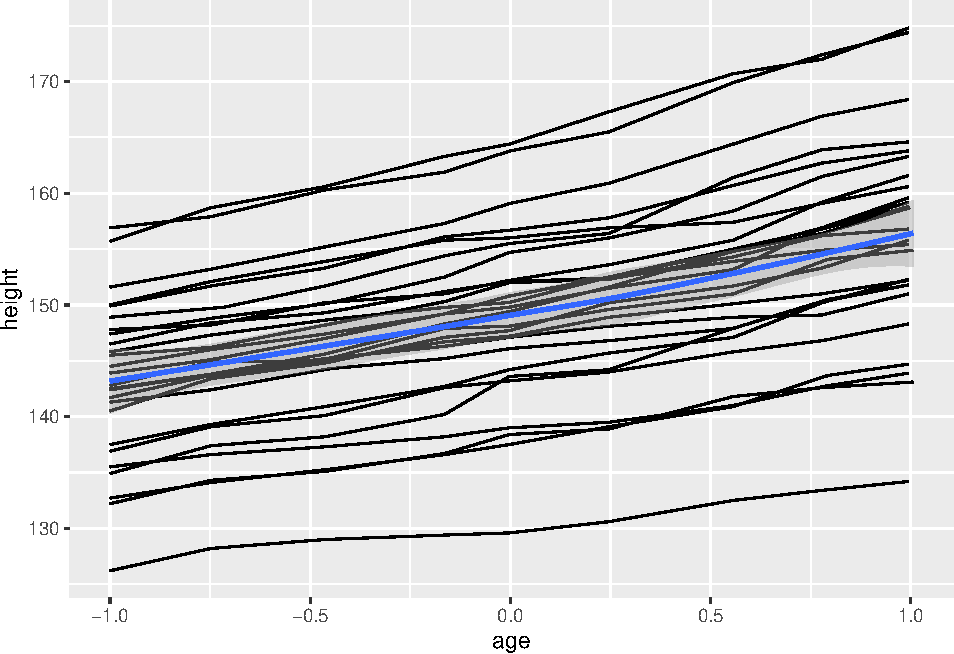
\includegraphics{Introduction-to-R,-Rstudio,-and-ggplot2_files/figure-latex/unnamed-chunk-36-1.pdf}

\begin{Shaded}
\begin{Highlighting}[]
\KeywordTok{ggplot}\NormalTok{(mpg, }\KeywordTok{aes}\NormalTok{(}\DataTypeTok{x =} \NormalTok{hwy, }\DataTypeTok{y =} \NormalTok{cty)) +}\StringTok{ }\KeywordTok{geom_point}\NormalTok{() +}\StringTok{ }\KeywordTok{theme_classic}\NormalTok{()}
\end{Highlighting}
\end{Shaded}

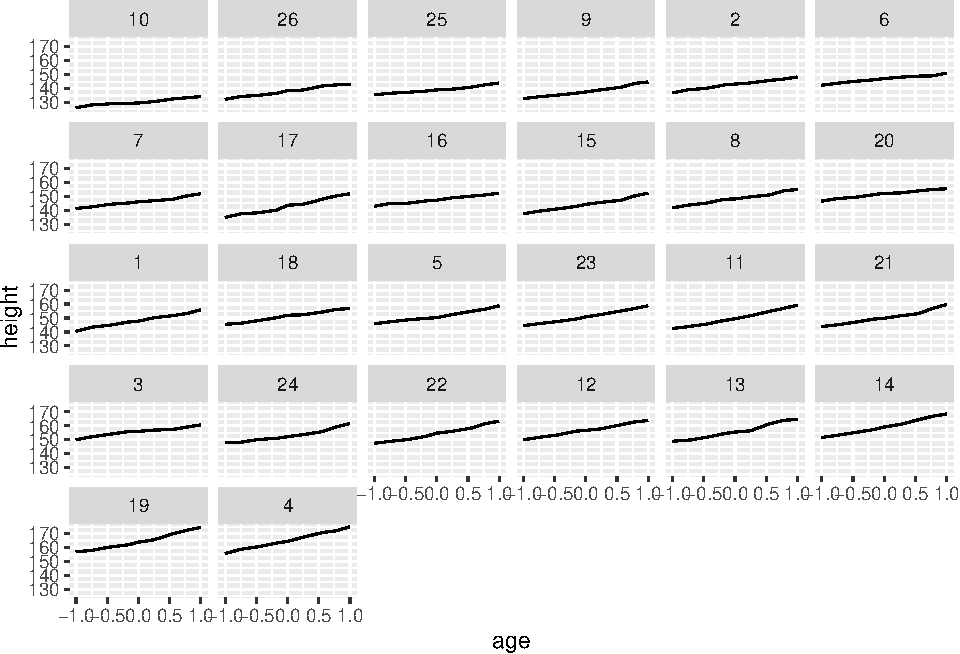
\includegraphics{Introduction-to-R,-Rstudio,-and-ggplot2_files/figure-latex/unnamed-chunk-37-1.pdf}

\section{Save a ggplot}\label{save-a-ggplot}

\begin{itemize}
\tightlist
\item
  \texttt{ggsave()} is a convenient function for saving a plot. It
  defaults to saving the \textbf{last plot} that you displayed.
\end{itemize}

\begin{Shaded}
\begin{Highlighting}[]
\KeywordTok{ggsave}\NormalTok{(}\StringTok{"mtcars.pdf"}\NormalTok{)}
\end{Highlighting}
\end{Shaded}

\begin{verbatim}
## Saving 6.5 x 4.5 in image
\end{verbatim}

\section{More resources}\label{more-resources}

\begin{itemize}
\tightlist
\item
  \texttt{ggplot2} Reference:
  \url{https://ggplot2.tidyverse.org/reference/index.html}
\item
  Many R galleries (e.g., \url{https://www.r-graph-gallery.com})
\item
  Google
\end{itemize}

\chapter{Descriptive Statistics}\label{descriptive-statistics}

\section{R functions for descriptive
statistics}\label{r-functions-for-descriptive-statistics}

\begin{Shaded}
\begin{Highlighting}[]
\CommentTok{# compute mean}
\CommentTok{# we use $ to access `price` variable in the `diamonds` dataset }
\KeywordTok{mean}\NormalTok{(diamonds$price)}
\end{Highlighting}
\end{Shaded}

\begin{verbatim}
## [1] 3932.8
\end{verbatim}

\begin{Shaded}
\begin{Highlighting}[]
\CommentTok{# compute median}
\KeywordTok{median}\NormalTok{(diamonds$price)}
\end{Highlighting}
\end{Shaded}

\begin{verbatim}
## [1] 2401
\end{verbatim}

\begin{Shaded}
\begin{Highlighting}[]
\CommentTok{# compute variance}
\KeywordTok{var}\NormalTok{(diamonds$price)}
\end{Highlighting}
\end{Shaded}

\begin{verbatim}
## [1] 15915629
\end{verbatim}

\begin{Shaded}
\begin{Highlighting}[]
\CommentTok{# compute standard deviation}
\KeywordTok{sd}\NormalTok{(diamonds$price)}
\end{Highlighting}
\end{Shaded}

\begin{verbatim}
## [1] 3989.44
\end{verbatim}

\begin{Shaded}
\begin{Highlighting}[]
\CommentTok{# summary of a data frame}
\KeywordTok{summary}\NormalTok{(diamonds)}
\end{Highlighting}
\end{Shaded}

\begin{verbatim}
##      carat               cut        color        clarity     
##  Min.   :0.2000   Fair     : 1610   D: 6775   SI1    :13065  
##  1st Qu.:0.4000   Good     : 4906   E: 9797   VS2    :12258  
##  Median :0.7000   Very Good:12082   F: 9542   SI2    : 9194  
##  Mean   :0.7979   Premium  :13791   G:11292   VS1    : 8171  
##  3rd Qu.:1.0400   Ideal    :21551   H: 8304   VVS2   : 5066  
##  Max.   :5.0100                     I: 5422   VVS1   : 3655  
##                                     J: 2808   (Other): 2531  
##      depth           table           price             x         
##  Min.   :43.00   Min.   :43.00   Min.   :  326   Min.   : 0.000  
##  1st Qu.:61.00   1st Qu.:56.00   1st Qu.:  950   1st Qu.: 4.710  
##  Median :61.80   Median :57.00   Median : 2401   Median : 5.700  
##  Mean   :61.75   Mean   :57.46   Mean   : 3933   Mean   : 5.731  
##  3rd Qu.:62.50   3rd Qu.:59.00   3rd Qu.: 5324   3rd Qu.: 6.540  
##  Max.   :79.00   Max.   :95.00   Max.   :18823   Max.   :10.740  
##                                                                  
##        y                z         
##  Min.   : 0.000   Min.   : 0.000  
##  1st Qu.: 4.720   1st Qu.: 2.910  
##  Median : 5.710   Median : 3.530  
##  Mean   : 5.735   Mean   : 3.539  
##  3rd Qu.: 6.540   3rd Qu.: 4.040  
##  Max.   :58.900   Max.   :31.800  
## 
\end{verbatim}

\section{qplot()}\label{qplot}

\texttt{qplot()}, short for \textbf{quick plot} is a function in the
\texttt{ggplot2} package. qplot makes it easy to produce complex plots,
often requiring several lines of code using other plotting systems,
\textbf{in one line}.

\section{Scatterplots}\label{scatterplots}

\begin{Shaded}
\begin{Highlighting}[]
\KeywordTok{ggplot}\NormalTok{(}\DataTypeTok{data =} \NormalTok{mpg, }\KeywordTok{aes}\NormalTok{(}\DataTypeTok{x =} \NormalTok{displ, }\DataTypeTok{y =} \NormalTok{hwy)) +}\StringTok{ }\KeywordTok{geom_point}\NormalTok{()}
\end{Highlighting}
\end{Shaded}

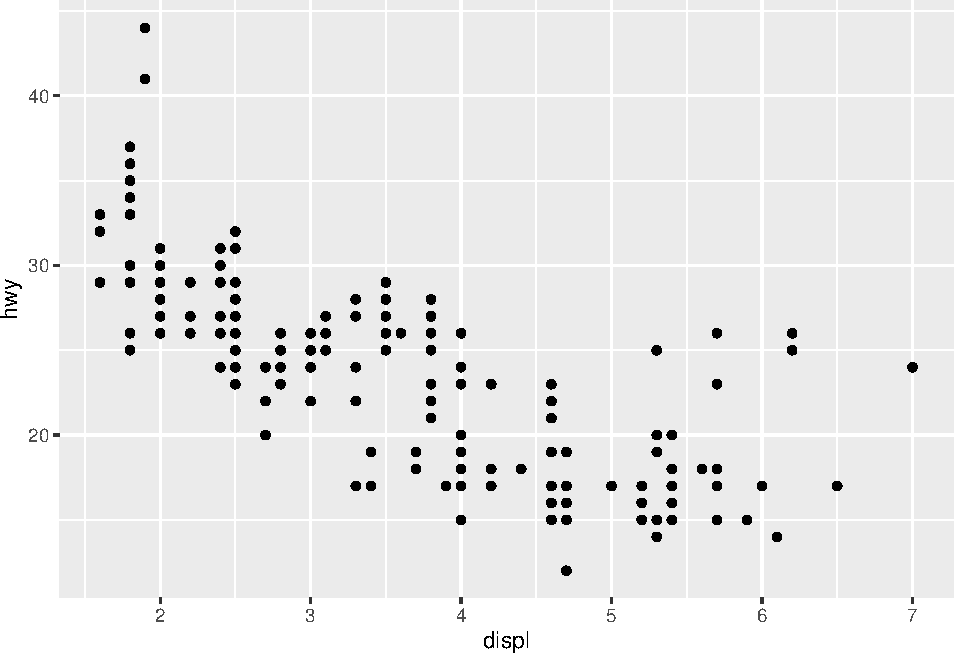
\includegraphics{Introduction-to-R,-Rstudio,-and-ggplot2_files/figure-latex/unnamed-chunk-44-1.pdf}

\begin{Shaded}
\begin{Highlighting}[]
\KeywordTok{qplot}\NormalTok{(displ, hwy, }\DataTypeTok{data =} \NormalTok{mpg)}
\end{Highlighting}
\end{Shaded}

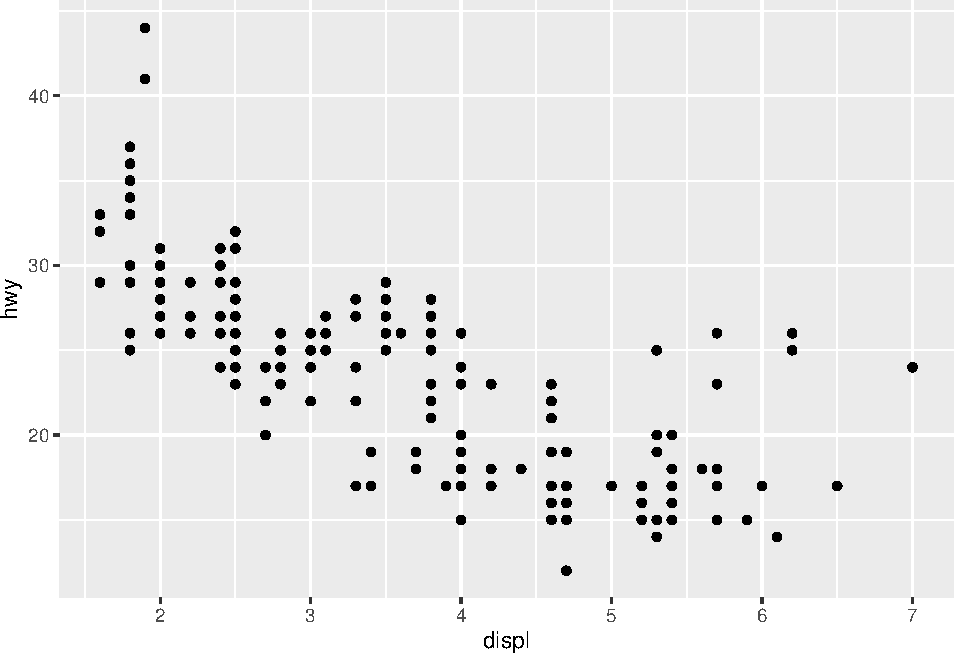
\includegraphics{Introduction-to-R,-Rstudio,-and-ggplot2_files/figure-latex/unnamed-chunk-45-1.pdf}

\begin{Shaded}
\begin{Highlighting}[]
\KeywordTok{ggplot}\NormalTok{(}\DataTypeTok{data =} \NormalTok{mpg, }\KeywordTok{aes}\NormalTok{(}\DataTypeTok{x =} \NormalTok{displ, }\DataTypeTok{y =} \NormalTok{hwy, }\DataTypeTok{color =} \NormalTok{class)) +}\StringTok{ }\KeywordTok{geom_point}\NormalTok{()}
\end{Highlighting}
\end{Shaded}

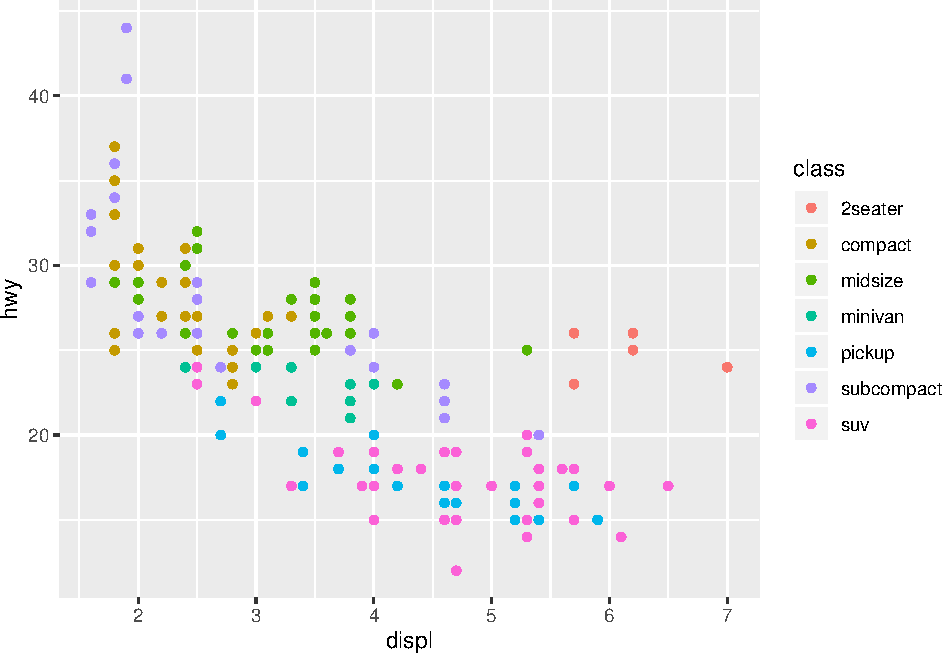
\includegraphics{Introduction-to-R,-Rstudio,-and-ggplot2_files/figure-latex/unnamed-chunk-46-1.pdf}

\begin{Shaded}
\begin{Highlighting}[]
\KeywordTok{qplot}\NormalTok{(displ, hwy, }\DataTypeTok{data =} \NormalTok{mpg, }\DataTypeTok{color =} \NormalTok{class)}
\end{Highlighting}
\end{Shaded}

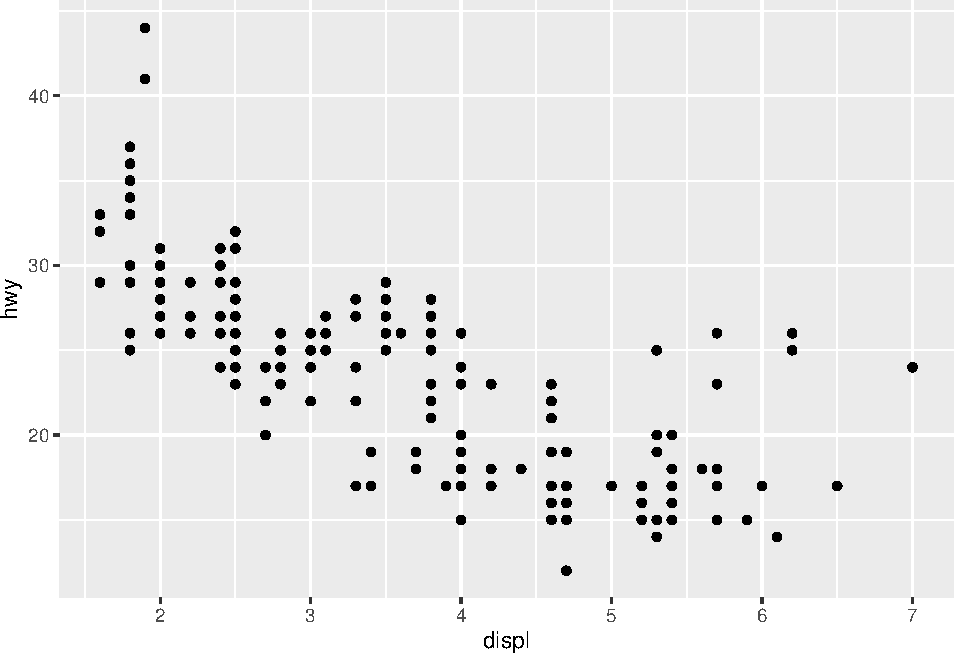
\includegraphics{Introduction-to-R,-Rstudio,-and-ggplot2_files/figure-latex/unnamed-chunk-47-1.pdf}

\begin{Shaded}
\begin{Highlighting}[]
\KeywordTok{ggplot}\NormalTok{(}\DataTypeTok{data =} \NormalTok{mpg, }\KeywordTok{aes}\NormalTok{(}\DataTypeTok{x =} \NormalTok{displ, }\DataTypeTok{y =} \NormalTok{hwy, }\DataTypeTok{color =} \NormalTok{class, }\DataTypeTok{shape =} \NormalTok{drv)) +}\StringTok{ }\KeywordTok{geom_point}\NormalTok{()}
\end{Highlighting}
\end{Shaded}

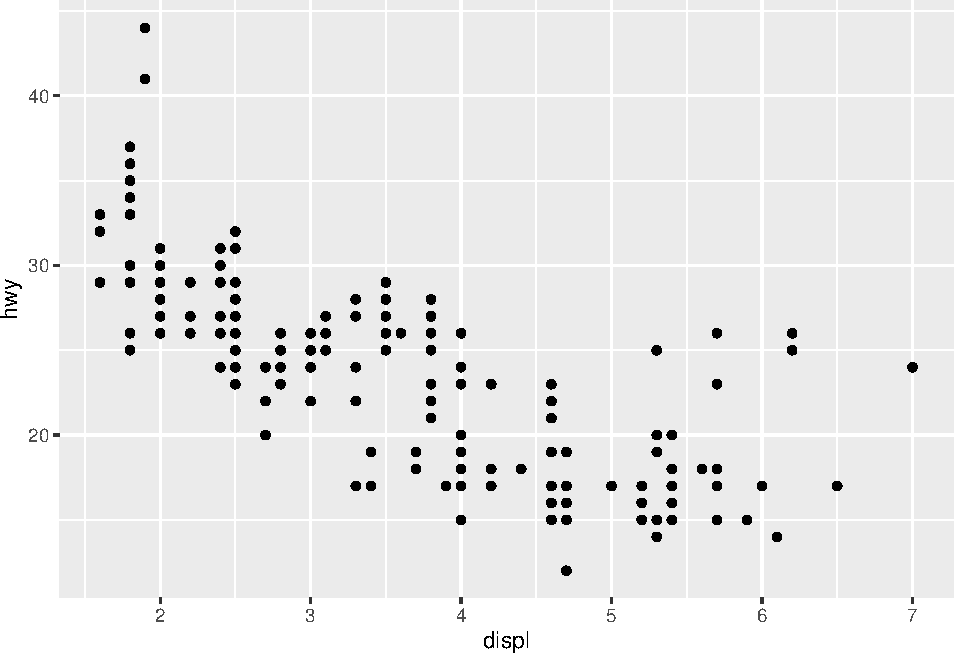
\includegraphics{Introduction-to-R,-Rstudio,-and-ggplot2_files/figure-latex/unnamed-chunk-48-1.pdf}

\begin{Shaded}
\begin{Highlighting}[]
\KeywordTok{qplot}\NormalTok{(displ, hwy, }\DataTypeTok{data =} \NormalTok{mpg, }\DataTypeTok{color =} \NormalTok{class, }\DataTypeTok{shape =} \NormalTok{drv)}
\end{Highlighting}
\end{Shaded}

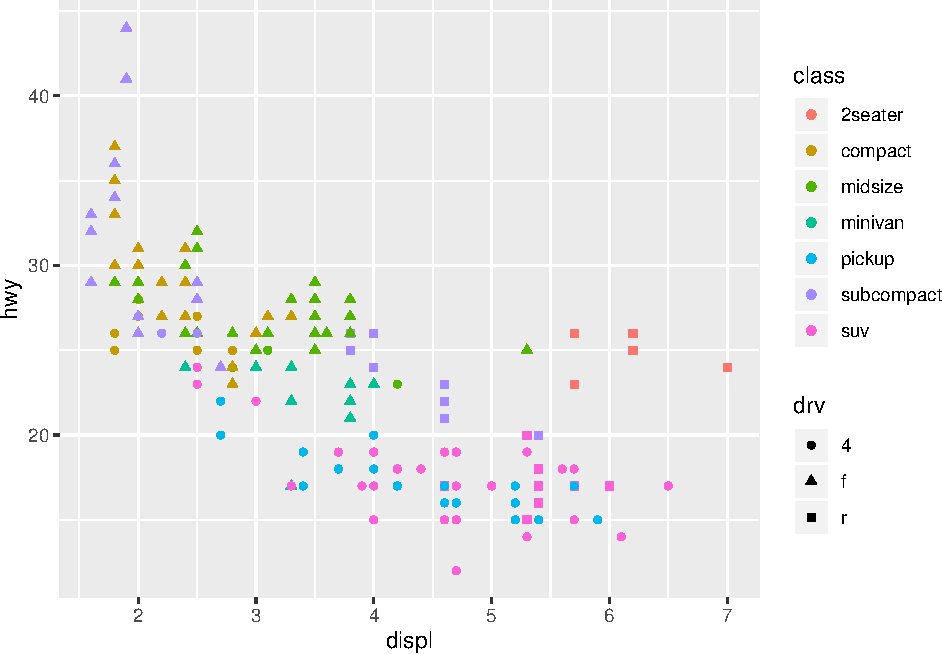
\includegraphics{Introduction-to-R,-Rstudio,-and-ggplot2_files/figure-latex/unnamed-chunk-49-1.pdf}

\begin{Shaded}
\begin{Highlighting}[]
\KeywordTok{ggplot}\NormalTok{(}\DataTypeTok{data =} \NormalTok{mpg, }\KeywordTok{aes}\NormalTok{(}\DataTypeTok{x =} \NormalTok{displ, }\DataTypeTok{y =} \NormalTok{hwy)) +}\StringTok{ }\KeywordTok{geom_point}\NormalTok{() +}\StringTok{ }\KeywordTok{geom_smooth}\NormalTok{(}\DataTypeTok{method =} \StringTok{"lm"}\NormalTok{)}
\end{Highlighting}
\end{Shaded}

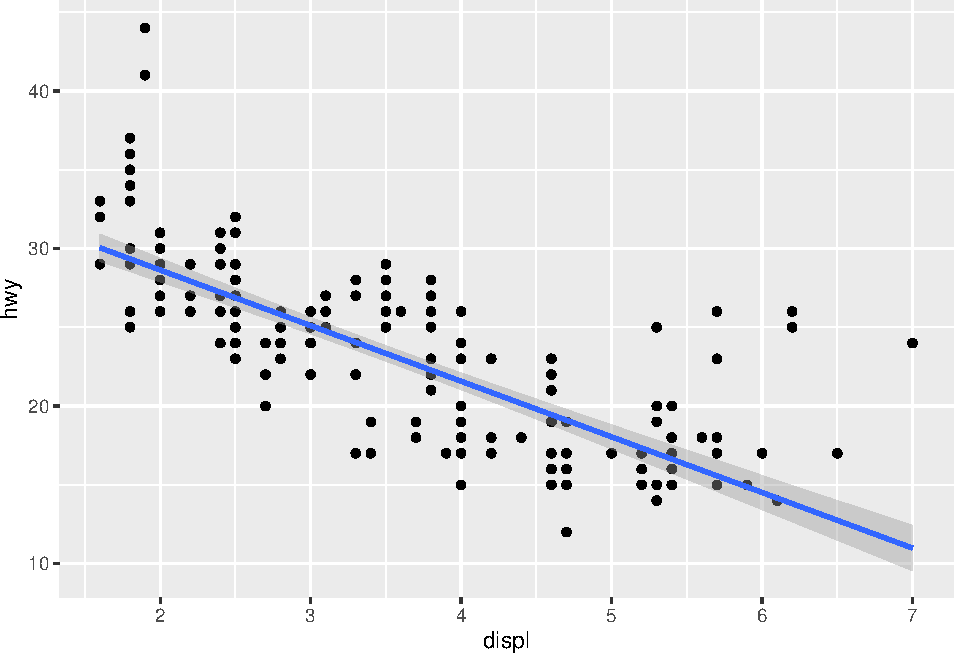
\includegraphics{Introduction-to-R,-Rstudio,-and-ggplot2_files/figure-latex/unnamed-chunk-50-1.pdf}

\begin{Shaded}
\begin{Highlighting}[]
\KeywordTok{qplot}\NormalTok{(displ, hwy, }\DataTypeTok{data =} \NormalTok{mpg, }\DataTypeTok{geom =} \KeywordTok{c}\NormalTok{(}\StringTok{"point"}\NormalTok{, }\StringTok{"smooth"}\NormalTok{)) }
\end{Highlighting}
\end{Shaded}

\begin{verbatim}
## `geom_smooth()` using method = 'loess' and formula 'y ~ x'
\end{verbatim}

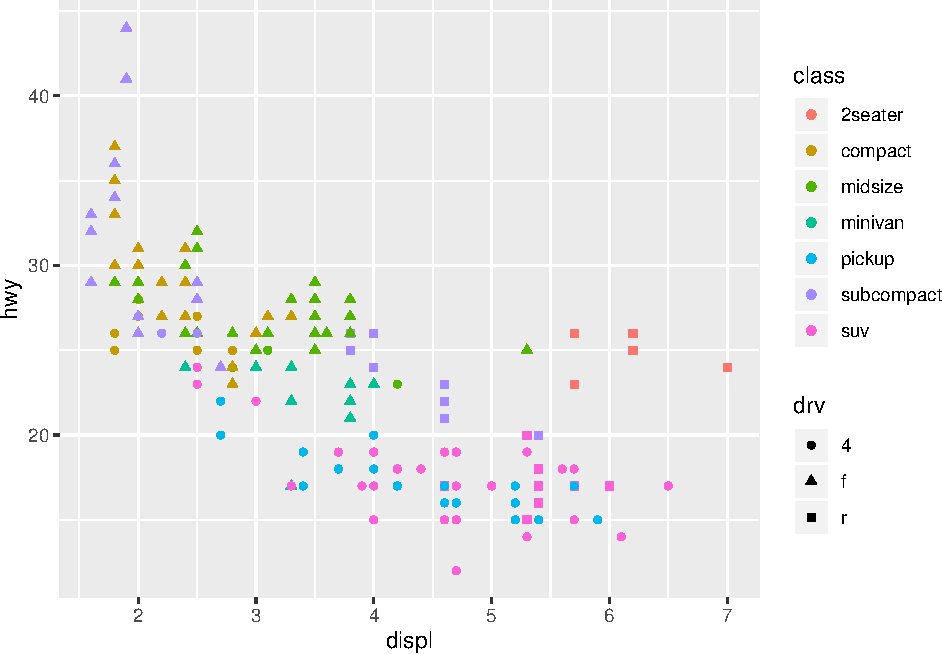
\includegraphics{Introduction-to-R,-Rstudio,-and-ggplot2_files/figure-latex/unnamed-chunk-51-1.pdf}

\section{Histogram}\label{histogram}

\begin{Shaded}
\begin{Highlighting}[]
\KeywordTok{ggplot}\NormalTok{(}\DataTypeTok{data =} \NormalTok{diamonds, }\KeywordTok{aes}\NormalTok{(}\DataTypeTok{x =} \NormalTok{carat)) +}\StringTok{ }\KeywordTok{geom_histogram}\NormalTok{()}
\end{Highlighting}
\end{Shaded}

\begin{verbatim}
## `stat_bin()` using `bins = 30`. Pick better value with `binwidth`.
\end{verbatim}

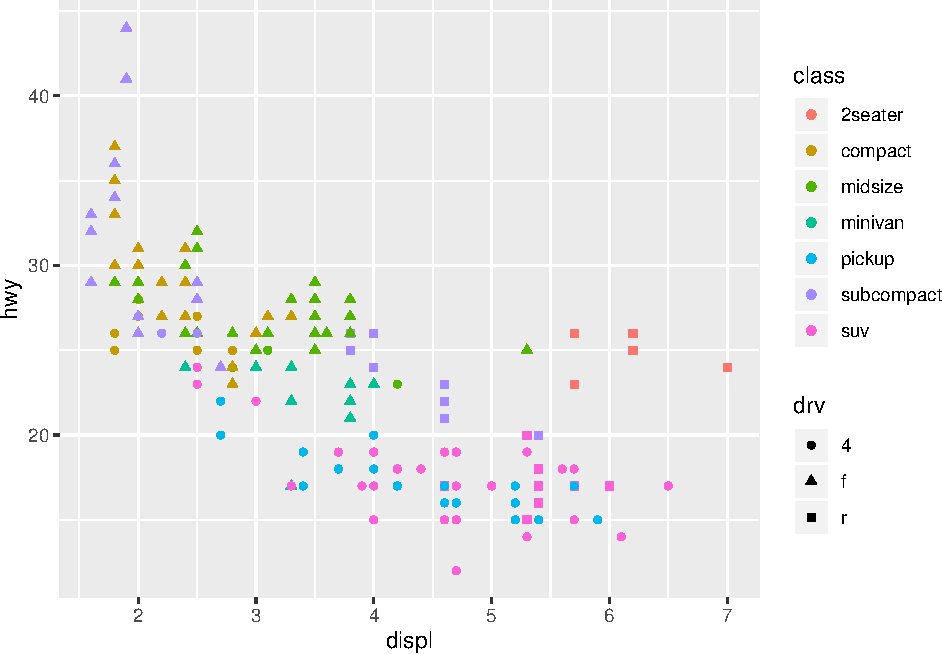
\includegraphics{Introduction-to-R,-Rstudio,-and-ggplot2_files/figure-latex/unnamed-chunk-52-1.pdf}

\begin{Shaded}
\begin{Highlighting}[]
\KeywordTok{qplot}\NormalTok{(carat, }\DataTypeTok{data =} \NormalTok{diamonds, }\DataTypeTok{geom =} \StringTok{"histogram"}\NormalTok{)}
\end{Highlighting}
\end{Shaded}

\begin{verbatim}
## `stat_bin()` using `bins = 30`. Pick better value with `binwidth`.
\end{verbatim}

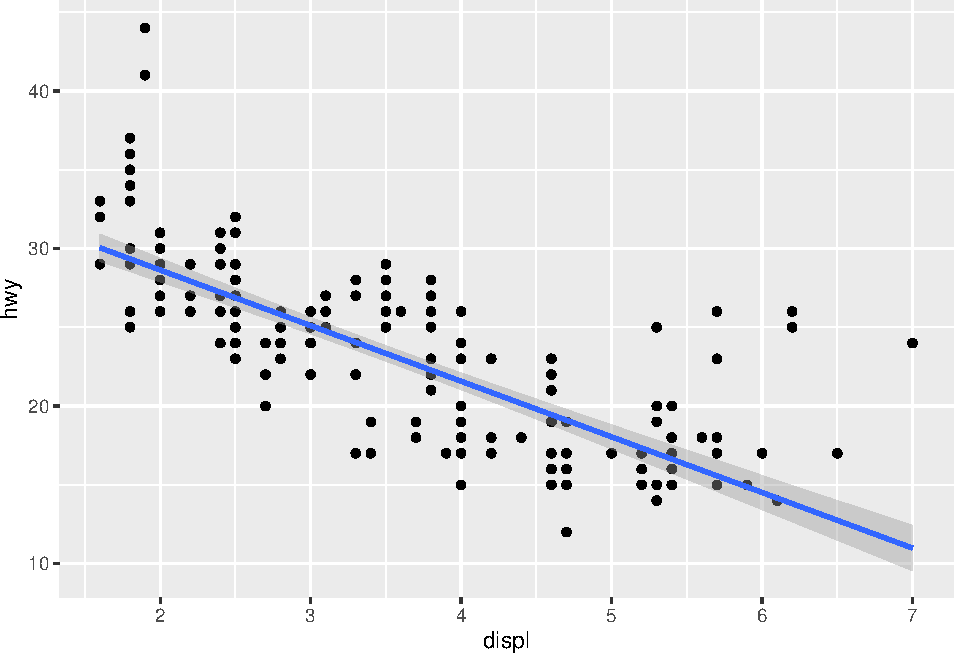
\includegraphics{Introduction-to-R,-Rstudio,-and-ggplot2_files/figure-latex/unnamed-chunk-53-1.pdf}

\begin{Shaded}
\begin{Highlighting}[]
\KeywordTok{ggplot}\NormalTok{(}\DataTypeTok{data =} \NormalTok{diamonds, }\KeywordTok{aes}\NormalTok{(}\DataTypeTok{x =} \NormalTok{carat)) +}\StringTok{ }\KeywordTok{geom_histogram}\NormalTok{(}\DataTypeTok{binwidth =} \FloatTok{0.05}\NormalTok{) +}\StringTok{ }\KeywordTok{xlim}\NormalTok{(}\KeywordTok{c}\NormalTok{(}\DecValTok{0}\NormalTok{,}\DecValTok{3}\NormalTok{))}
\end{Highlighting}
\end{Shaded}

\begin{verbatim}
## Warning: Removed 32 rows containing non-finite values (stat_bin).
\end{verbatim}

\begin{verbatim}
## Warning: Removed 2 rows containing missing values (geom_bar).
\end{verbatim}

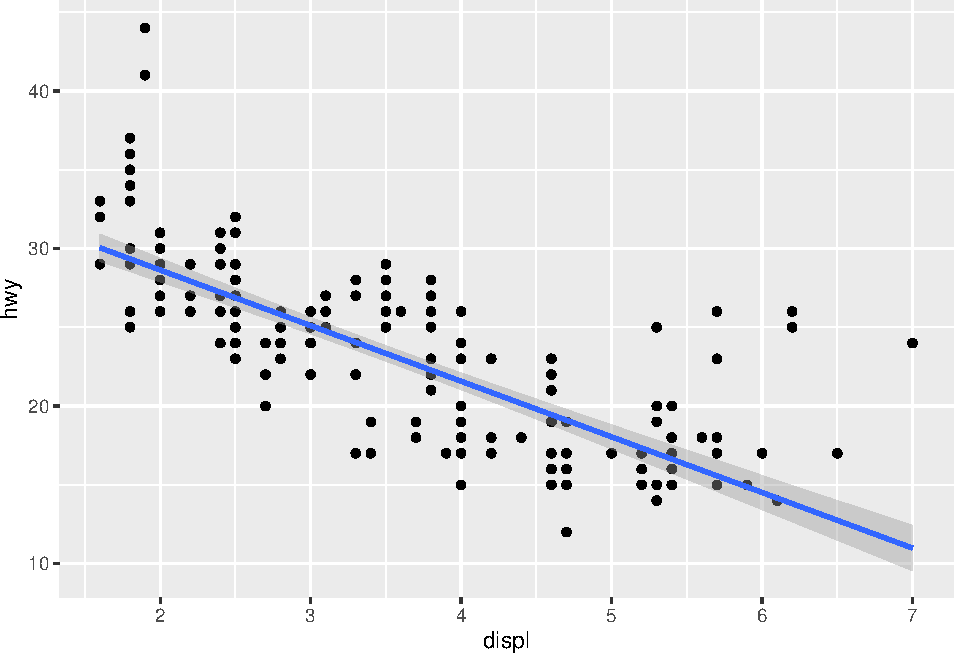
\includegraphics{Introduction-to-R,-Rstudio,-and-ggplot2_files/figure-latex/unnamed-chunk-54-1.pdf}

\begin{Shaded}
\begin{Highlighting}[]
\KeywordTok{qplot}\NormalTok{(carat, }\DataTypeTok{data =} \NormalTok{diamonds, }\DataTypeTok{geom =} \StringTok{"histogram"}\NormalTok{, }\DataTypeTok{binwidth =} \FloatTok{0.05}\NormalTok{, }\DataTypeTok{xlim =} \KeywordTok{c}\NormalTok{(}\DecValTok{0}\NormalTok{,}\DecValTok{3}\NormalTok{))}
\end{Highlighting}
\end{Shaded}

\begin{verbatim}
## Warning: Removed 32 rows containing non-finite values (stat_bin).
\end{verbatim}

\begin{verbatim}
## Warning: Removed 2 rows containing missing values (geom_bar).
\end{verbatim}

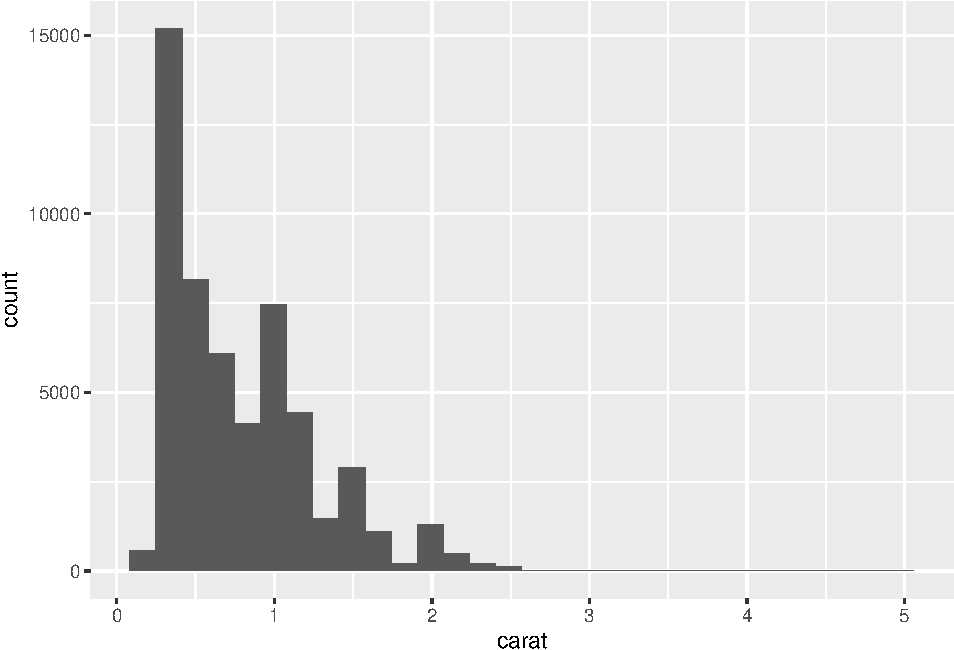
\includegraphics{Introduction-to-R,-Rstudio,-and-ggplot2_files/figure-latex/unnamed-chunk-55-1.pdf}

\begin{Shaded}
\begin{Highlighting}[]
\KeywordTok{ggplot}\NormalTok{(}\DataTypeTok{data =} \NormalTok{mpg, }\KeywordTok{aes}\NormalTok{(}\DataTypeTok{x =} \NormalTok{hwy, }\DataTypeTok{fill =} \NormalTok{drv)) +}\StringTok{ }\KeywordTok{geom_histogram}\NormalTok{() }
\end{Highlighting}
\end{Shaded}

\begin{verbatim}
## `stat_bin()` using `bins = 30`. Pick better value with `binwidth`.
\end{verbatim}

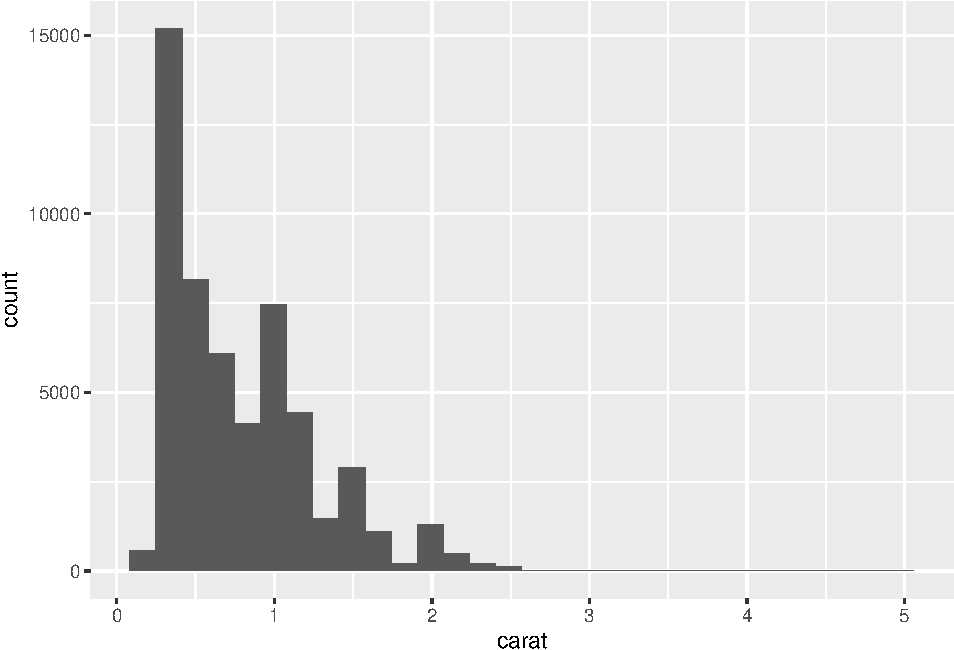
\includegraphics{Introduction-to-R,-Rstudio,-and-ggplot2_files/figure-latex/unnamed-chunk-56-1.pdf}

\begin{Shaded}
\begin{Highlighting}[]
\KeywordTok{qplot}\NormalTok{(hwy, }\DataTypeTok{data =} \NormalTok{mpg, }\DataTypeTok{geom =} \StringTok{"histogram"}\NormalTok{, }\DataTypeTok{fill =} \NormalTok{drv)}
\end{Highlighting}
\end{Shaded}

\begin{verbatim}
## `stat_bin()` using `bins = 30`. Pick better value with `binwidth`.
\end{verbatim}

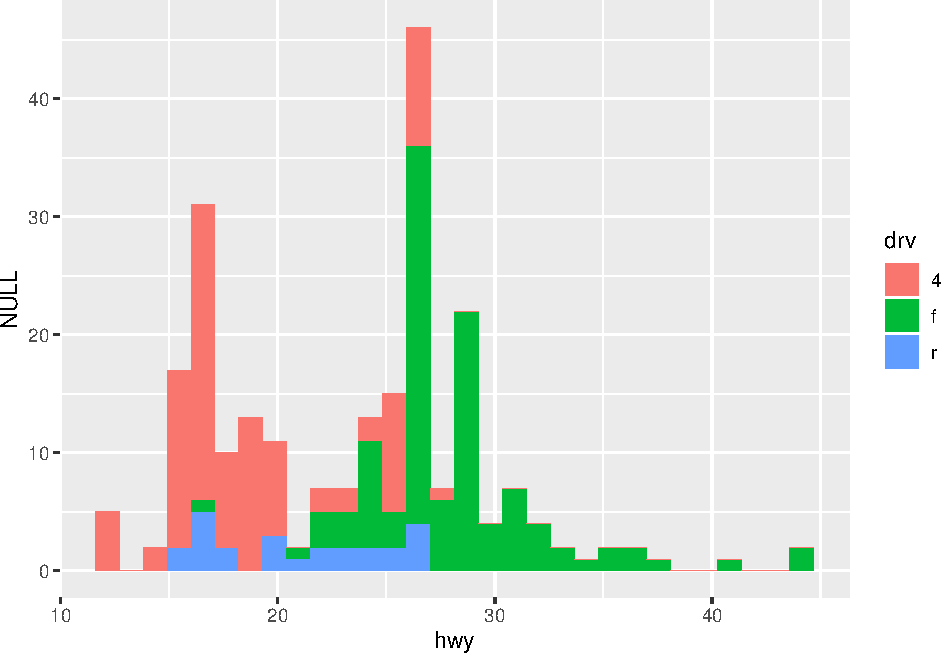
\includegraphics{Introduction-to-R,-Rstudio,-and-ggplot2_files/figure-latex/unnamed-chunk-57-1.pdf}

\section{Density plots}\label{density-plots}

\begin{Shaded}
\begin{Highlighting}[]
\KeywordTok{ggplot}\NormalTok{(}\DataTypeTok{data =} \NormalTok{diamonds, }\KeywordTok{aes}\NormalTok{(}\DataTypeTok{x =} \NormalTok{carat, }\DataTypeTok{color =} \NormalTok{color)) +}\StringTok{ }\KeywordTok{geom_density}\NormalTok{() }
\end{Highlighting}
\end{Shaded}

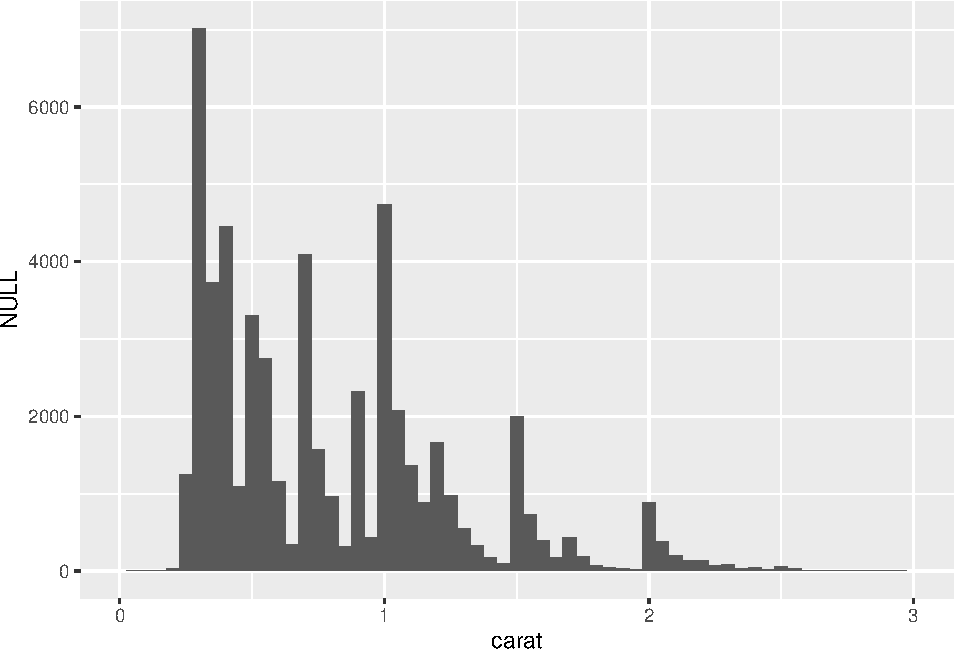
\includegraphics{Introduction-to-R,-Rstudio,-and-ggplot2_files/figure-latex/unnamed-chunk-58-1.pdf}

\begin{Shaded}
\begin{Highlighting}[]
\KeywordTok{qplot}\NormalTok{(carat, }\DataTypeTok{data =} \NormalTok{diamonds, }\DataTypeTok{geom =} \StringTok{"density"}\NormalTok{, }\DataTypeTok{color =} \NormalTok{color)}
\end{Highlighting}
\end{Shaded}

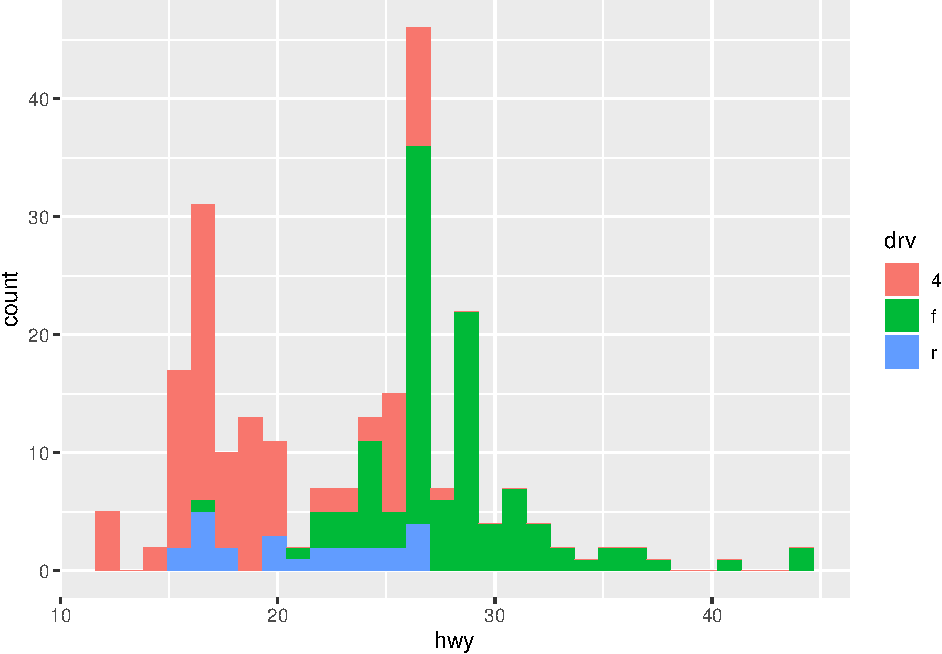
\includegraphics{Introduction-to-R,-Rstudio,-and-ggplot2_files/figure-latex/unnamed-chunk-59-1.pdf}

\section{Barplots}\label{barplots}

\begin{Shaded}
\begin{Highlighting}[]
\KeywordTok{ggplot}\NormalTok{(}\DataTypeTok{data =} \NormalTok{diamonds, }\KeywordTok{aes}\NormalTok{(}\DataTypeTok{x =} \NormalTok{clarity)) +}\StringTok{ }\KeywordTok{geom_bar}\NormalTok{() }
\end{Highlighting}
\end{Shaded}

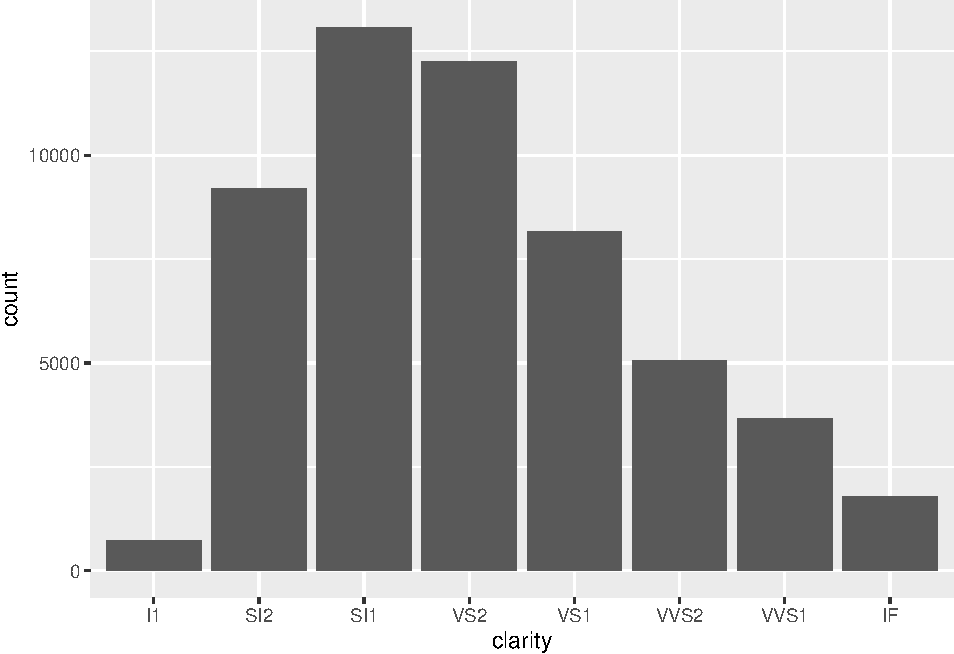
\includegraphics{Introduction-to-R,-Rstudio,-and-ggplot2_files/figure-latex/unnamed-chunk-60-1.pdf}

\begin{Shaded}
\begin{Highlighting}[]
\KeywordTok{qplot}\NormalTok{(clarity, }\DataTypeTok{data =} \NormalTok{diamonds, }\DataTypeTok{geom =} \StringTok{"bar"}\NormalTok{)}
\end{Highlighting}
\end{Shaded}

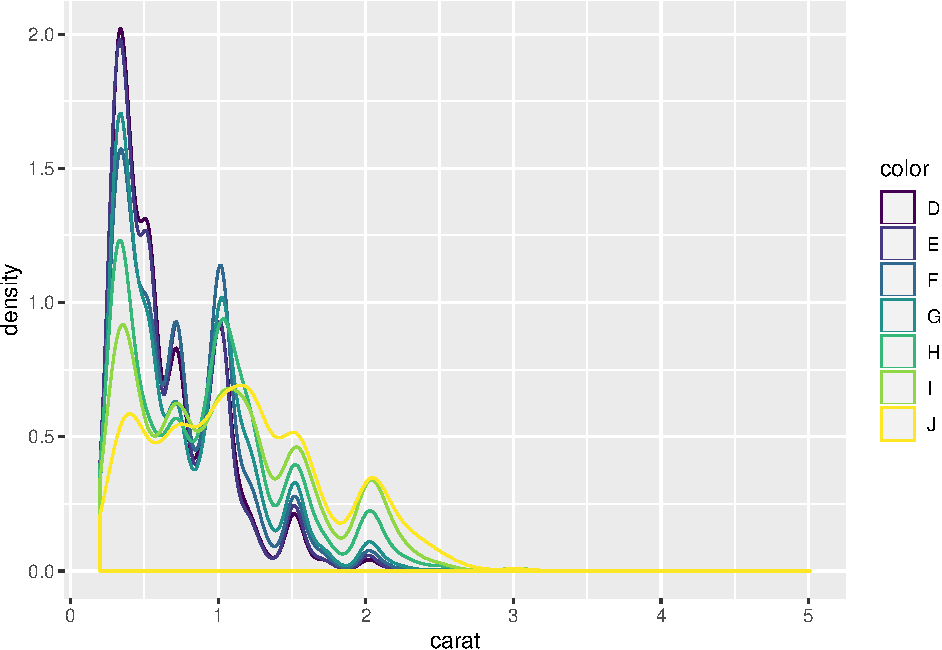
\includegraphics{Introduction-to-R,-Rstudio,-and-ggplot2_files/figure-latex/unnamed-chunk-61-1.pdf}

\begin{Shaded}
\begin{Highlighting}[]
\KeywordTok{ggplot}\NormalTok{(}\DataTypeTok{data =} \NormalTok{diamonds, }\KeywordTok{aes}\NormalTok{(}\DataTypeTok{x =} \NormalTok{clarity, }\DataTypeTok{fill =} \NormalTok{cut)) +}\StringTok{ }\KeywordTok{geom_bar}\NormalTok{() }
\end{Highlighting}
\end{Shaded}

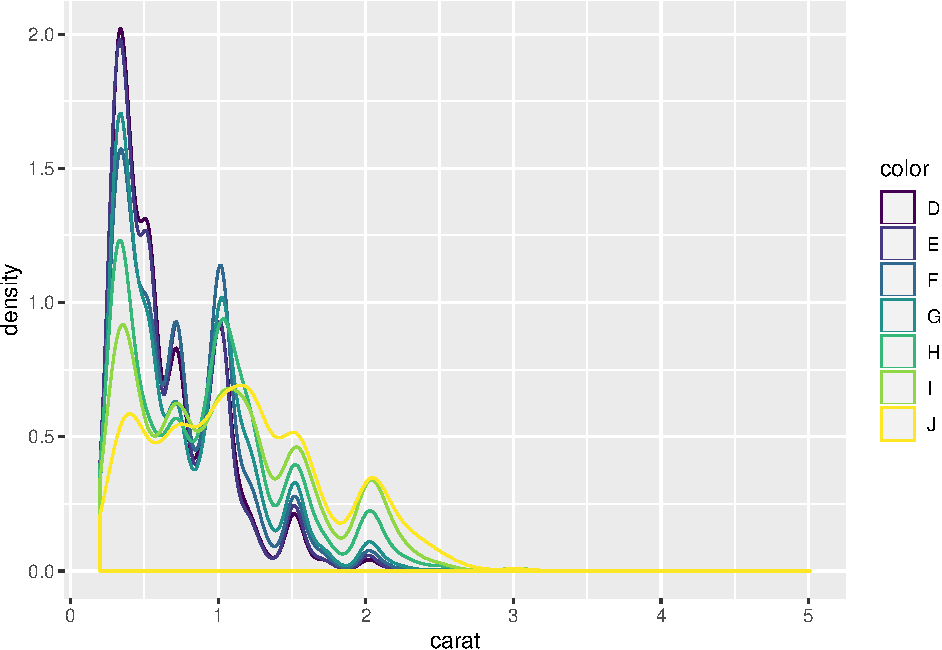
\includegraphics{Introduction-to-R,-Rstudio,-and-ggplot2_files/figure-latex/unnamed-chunk-62-1.pdf}

\begin{Shaded}
\begin{Highlighting}[]
\KeywordTok{qplot}\NormalTok{(clarity, }\DataTypeTok{data =} \NormalTok{diamonds, }\DataTypeTok{geom =} \StringTok{"bar"}\NormalTok{, }\DataTypeTok{fill =} \NormalTok{cut)}
\end{Highlighting}
\end{Shaded}

\includegraphics{Introduction-to-R,-Rstudio,-and-ggplot2_files/figure-latex/unnamed-chunk-63-1.pdf}

\section{Boxplots}\label{boxplots}

\begin{Shaded}
\begin{Highlighting}[]
\KeywordTok{ggplot}\NormalTok{(}\DataTypeTok{data =} \NormalTok{diamonds, }\KeywordTok{aes}\NormalTok{(}\DataTypeTok{y =} \NormalTok{price)) +}\StringTok{ }\KeywordTok{geom_boxplot}\NormalTok{() }
\end{Highlighting}
\end{Shaded}

\includegraphics{Introduction-to-R,-Rstudio,-and-ggplot2_files/figure-latex/unnamed-chunk-64-1.pdf}

\begin{Shaded}
\begin{Highlighting}[]
\KeywordTok{qplot}\NormalTok{(}\DataTypeTok{y =} \NormalTok{price, }\DataTypeTok{data =} \NormalTok{diamonds, }\DataTypeTok{geom =} \StringTok{"boxplot"}\NormalTok{)}
\end{Highlighting}
\end{Shaded}

\includegraphics{Introduction-to-R,-Rstudio,-and-ggplot2_files/figure-latex/unnamed-chunk-65-1.pdf}

\begin{Shaded}
\begin{Highlighting}[]
\KeywordTok{ggplot}\NormalTok{(}\DataTypeTok{data =} \NormalTok{diamonds, }\KeywordTok{aes}\NormalTok{(}\DataTypeTok{x =} \NormalTok{cut, }\DataTypeTok{y =} \NormalTok{price)) +}\StringTok{ }\KeywordTok{geom_boxplot}\NormalTok{() }
\end{Highlighting}
\end{Shaded}

\includegraphics{Introduction-to-R,-Rstudio,-and-ggplot2_files/figure-latex/unnamed-chunk-66-1.pdf}

\section{Faceting}\label{faceting}

\begin{Shaded}
\begin{Highlighting}[]
\KeywordTok{ggplot}\NormalTok{(}\DataTypeTok{data =} \NormalTok{diamonds, }\KeywordTok{aes}\NormalTok{(}\DataTypeTok{x =} \NormalTok{carat, }\DataTypeTok{y =} \NormalTok{price)) +}\StringTok{ }\KeywordTok{geom_point}\NormalTok{() +}\StringTok{ }\KeywordTok{facet_grid}\NormalTok{(cut ~}\StringTok{ }\NormalTok{color)}
\end{Highlighting}
\end{Shaded}

\includegraphics{Introduction-to-R,-Rstudio,-and-ggplot2_files/figure-latex/unnamed-chunk-67-1.pdf}

\begin{Shaded}
\begin{Highlighting}[]
\KeywordTok{qplot}\NormalTok{(carat, price, }\DataTypeTok{data =} \NormalTok{diamonds, }\DataTypeTok{facets =} \NormalTok{cut ~}\StringTok{ }\NormalTok{color)}
\end{Highlighting}
\end{Shaded}

\includegraphics{Introduction-to-R,-Rstudio,-and-ggplot2_files/figure-latex/unnamed-chunk-68-1.pdf}

\section{\texorpdfstring{The \texttt{corrplot}
Package}{The corrplot Package}}\label{the-corrplot-package}

\begin{itemize}
\tightlist
\item
  \url{https://cran.r-project.org/web/packages/corrplot/vignettes/corrplot-intro.html}
\item
  ``The corrplot package is a graphical display of a \textbf{correlation
  matrix}, confidence interval. It also contains some algorithms to do
  matrix reordering. In addition, corrplot is good at details, including
  choosing color, text labels, color labels, layout, etc.''
\end{itemize}

\begin{Shaded}
\begin{Highlighting}[]
\KeywordTok{library}\NormalTok{(corrplot)}
\end{Highlighting}
\end{Shaded}

\begin{Shaded}
\begin{Highlighting}[]
\KeywordTok{corrplot.mixed}\NormalTok{(}\KeywordTok{cor}\NormalTok{(mtcars))}
\end{Highlighting}
\end{Shaded}

\includegraphics{Introduction-to-R,-Rstudio,-and-ggplot2_files/figure-latex/unnamed-chunk-70-1.pdf}

\chapter{Exercise}\label{exercise-3}

\begin{itemize}
\tightlist
\item
  Exercise 1: \texttt{midwest} is a dataset in \texttt{ggplot2}, and
  contains demographic information of midwest counties. Replicate the
  following scatterplot as close as you can. The variable for the
  x-axis, y-axis, color aesthetic, size aesthetic are \texttt{area},
  \texttt{poptotal}, \texttt{state}, and \texttt{popdensity}.
\end{itemize}

\begin{figure}[htbp]
\centering
\includegraphics{practice1.png}
\caption{}
\end{figure}

\begin{itemize}
\tightlist
\item
  Excercise 2: Replicate the following barplot using the \texttt{mpg}
  dataset. Use
  \texttt{theme(axis.text.x\ =\ element\_text(angle=65,\ vjust=0.6))}.
  Check why we need this theme by plotting with and without this theme.
  You also need \texttt{width\ =\ 0.5} option in a geom to have more
  space between bar.
\end{itemize}

\begin{figure}[htbp]
\centering
\includegraphics{practice2.png}
\caption{}
\end{figure}

\begin{itemize}
\tightlist
\item
  Excercise 3: Replicate the following density plot using the
  \texttt{mpg} dataset. You need an \texttt{alpha} aesthetic to make
  densities transparent.
\end{itemize}

\begin{figure}[htbp]
\centering
\includegraphics{practice3.png}
\caption{}
\end{figure}

\bibliography{book.bib}


\end{document}
